\batchmode
\documentclass[twoside]{article}

% Packages required by doxygen
\usepackage{fixltx2e}
\usepackage{calc}
\usepackage{doxygen}
\usepackage[export]{adjustbox} % also loads graphicx
\usepackage{graphicx}
\usepackage[utf8]{inputenc}
\usepackage{makeidx}
\usepackage{multicol}
\usepackage{multirow}
\PassOptionsToPackage{warn}{textcomp}
\usepackage{textcomp}
\usepackage[nointegrals]{wasysym}
\usepackage[table]{xcolor}

% Font selection
\usepackage[T1]{fontenc}
\usepackage[scaled=.90]{helvet}
\usepackage{courier}
\usepackage{amssymb}
\usepackage{sectsty}
\renewcommand{\familydefault}{\sfdefault}
\allsectionsfont{%
  \fontseries{bc}\selectfont%
  \color{darkgray}%
}
\renewcommand{\DoxyLabelFont}{%
  \fontseries{bc}\selectfont%
  \color{darkgray}%
}
\newcommand{\+}{\discretionary{\mbox{\scriptsize$\hookleftarrow$}}{}{}}

% Page & text layout
\usepackage{geometry}
\geometry{%
  a4paper,%
  top=2.5cm,%
  bottom=2.5cm,%
  left=2.5cm,%
  right=2.5cm%
}
\tolerance=750
\hfuzz=15pt
\hbadness=750
\setlength{\emergencystretch}{15pt}
\setlength{\parindent}{0cm}
\setlength{\parskip}{0.2cm}
\makeatletter
\renewcommand{\paragraph}{%
  \@startsection{paragraph}{4}{0ex}{-1.0ex}{1.0ex}{%
    \normalfont\normalsize\bfseries\SS@parafont%
  }%
}
\renewcommand{\subparagraph}{%
  \@startsection{subparagraph}{5}{0ex}{-1.0ex}{1.0ex}{%
    \normalfont\normalsize\bfseries\SS@subparafont%
  }%
}
\makeatother

% Headers & footers
\usepackage{fancyhdr}
\pagestyle{fancyplain}
\fancyhead[LE]{\fancyplain{}{\bfseries\thepage}}
\fancyhead[CE]{\fancyplain{}{}}
\fancyhead[RE]{\fancyplain{}{\bfseries\leftmark}}
\fancyhead[LO]{\fancyplain{}{\bfseries\rightmark}}
\fancyhead[CO]{\fancyplain{}{}}
\fancyhead[RO]{\fancyplain{}{\bfseries\thepage}}
\fancyfoot[LE]{\fancyplain{}{}}
\fancyfoot[CE]{\fancyplain{}{}}
\fancyfoot[RE]{\fancyplain{}{\bfseries\scriptsize Generated on Mon Dec 14 2015 09\+:32\+:11 for libridc-\/0.\+2 by Doxygen }}
\fancyfoot[LO]{\fancyplain{}{\bfseries\scriptsize Generated on Mon Dec 14 2015 09\+:32\+:11 for libridc-\/0.\+2 by Doxygen }}
\fancyfoot[CO]{\fancyplain{}{}}
\fancyfoot[RO]{\fancyplain{}{}}
\renewcommand{\footrulewidth}{0.4pt}
\renewcommand{\sectionmark}[1]{%
  \markright{\thesection\ #1}%
}

% Indices & bibliography
\usepackage{natbib}
\usepackage[titles]{tocloft}
\setcounter{tocdepth}{3}
\setcounter{secnumdepth}{5}
\makeindex

% Custom commands
\newcommand{\clearemptydoublepage}{%
  \newpage{\pagestyle{empty}\cleardoublepage}%
}


%===== C O N T E N T S =====

\begin{document}

% Titlepage & ToC
\pagenumbering{roman}
\begin{titlepage}
\vspace*{7cm}
\begin{center}%
{\Large libridc-\/0.2 }\\
\vspace*{1cm}
{\large Generated by Doxygen 1.8.10}\\
\vspace*{0.5cm}
{\small Mon Dec 14 2015 09:32:11}\\
\end{center}
\end{titlepage}
\tableofcontents
\pagenumbering{arabic}

%--- Begin generated contents ---
\section{About R\+I\+D\+C}
\label{md_README}
Revisionist Integral Deferred Correction methods -- a family of high-\/order, parallel time-\/integrators.

Revisionist integral deferred correction (R\+I\+D\+C) methods are a family of parallel--in--time methods to solve systems of initial values problems. The approach is able to bootstrap lower order time integrators to provide high order approximations in approximately the same wall clock time, hence providing a multiplicative increase in the number of compute cores utilized. Here we provide a C++ framework which automatically produces a parallel--in--time solution of a system of initial value problems given user supplied code for the right hand side of the system and a sequential code for a first-\/order time step. The user supplied time step routine may be explicit or implicit and may make use of any auxiliary libraries which take care of the solution of any nonlinear algebraic systems which may arise or the numerical linear algebra required. The code contains six examples of increasing complexity which also serve as templates to solve user defined problems. 
\section{Building and Installing}
\label{md_doc_source_0_installing}
\subsubsection*{Prerequisites}

There are no prerequisites for building the base R\+I\+D\+C software and examples in {\ttfamily explicit/} and {\ttfamily implicit/}. To build the example in {\ttfamily brusselator\+\_\+gsl/}, the G\+N\+U Scientific Library and headers need to be installed. To build examples in {\ttfamily implicit\+\_\+mkl/}, {\ttfamily brusselator\+\_\+mkl/} and {\ttfamily brusselator\textbackslash{}\+\_\+radau\textbackslash{}\+\_\+mkl/}, the Intel Math Kernel Library needs to be installed, and appropriate environment variables initialized.

\paragraph*{Required}


\begin{DoxyItemize}
\item A recent C++ compiler that supports (most of) the C++11 standard. This code has been successfully tested with G\+C\+C 4.\+1.\+x and the Intel Compiler 13.\+0.\+x.
\end{DoxyItemize}

\paragraph*{Optional}


\begin{DoxyItemize}
\item Intel M\+K\+L or G\+N\+U Scientific Library are required for some of the examples.
\end{DoxyItemize}

\subsubsection*{Obtain the Source Code}

The R\+I\+D\+C software is hosted at {\tt http\+://mathgeek.\+us/software.\+html}. Users should download the latest {\ttfamily libridc-\/x.\+x.\+tar.\+gz}, and uncompress the file to your desired location.

\subsubsection*{Configure the Software}

In the top level directory, {\ttfamily ./configure -\/-\/help} gives the possible configuration options. To configure using standard build configuration, type {\ttfamily ./configure -\/-\/prefix=/home/user/opt/libridc}. If you wish to compile and check the M\+K\+L and G\+S\+L examples, add the configuration flags {\ttfamily -\/-\/with-\/intel-\/mkl} or {\ttfamily -\/-\/with-\/gsl} respectively.

\subsubsection*{Building with Software}

The library is built by typing {\ttfamily make \&\& make check \&\& make install}. By default, only the explicit and implicit examples are part of make check, unless the {\ttfamily -\/-\/with-\/intel-\/mkl} or {\ttfamily -\/-\/with-\/gsl} flags are added in the configuration step. 
\section{Contributing}
\label{page_contributing}
The R\+I\+D\+C software is managed by the G\+N\+U build system. As such, the developer release requires G\+N\+U autoconf, automake, libtool, m4, make and their respective prerequisites. If there are version mismatches between the R\+I\+D\+C software and the local system, issuing the commands {\ttfamily autoreconf -\/f} and {\ttfamily automake -\/a -\/c} should resolve version errors and warning. To build the documentation, Doxygen must be installed, as well as appropriate Doxygen pre-\/requisites. For example, to build a P\+D\+F manual documenting the source code, Doxygen requires a La\+Te\+X compiler.

\subsubsection*{Branching}

Contributors should fork the git repository hosted at {\tt https\+://github.\+com/ongbw/ridc.\+git}

If this project gets large enough, we will utilize the {\tt git-\/flow} workflow

\begin{TabularC}{2}
\hline
\rowcolor{lightgray}{\bf Branch Name Pattern }&{\bf Description  }\\\cline{1-2}
{\ttfamily master} &tip of the {\ttfamily master} branch is always the latest stable release \\\cline{1-2}
{\ttfamily development} &tip of the {\ttfamily development} branch is the current state of development and not expected to be stable or even usable \\\cline{1-2}
{\ttfamily feature/$\ast$} &various feature branches are used to implement new features and should be based off the {\ttfamily development} branch \\\cline{1-2}
{\ttfamily release/$\ast$} &a release branch is created from the {\ttfamily development} branch and used to prepare a new release and will be merged into {\ttfamily master} \\\cline{1-2}
{\ttfamily hotfix/$\ast$} &hotfix branches are based off {\ttfamily master} or {\ttfamily development} to fix important and severe bugs and should be merged into {\ttfamily development} and {\ttfamily master} as soon as possible \\\cline{1-2}
\end{TabularC}
Releases and release candidates are tagged in the form {\ttfamily release-\/\+X.\+Y.\+Z(-\/\+R\+Ca)}, where {\ttfamily X}, {\ttfamily Y}, and {\ttfamily Z} specify the version with respect to [semantic versioning] and {\ttfamily a} the number of the release candidate of that version.

\subsubsection*{Commit Messages}

Please keep commit messages clean and descriptive as possible. The following are suggested\+:


\begin{DoxyItemize}
\item Commit Title must not be longer than 50 characters

If applicable, the title should start with a category name (such as {\ttfamily docu}, {\ttfamily tests}, ...) followed by a colon (e.\+g. {\ttfamily \char`\"{}docu\+: add usage
  examples for R\+I\+D\+C\char`\"{}} ).
\item Commit Description must have line wraps at 72 characters
\item Please {\itshape sign} your commits (i.\+e. use {\ttfamily git commit -\/s})
\end{DoxyItemize}

\subsubsection*{How to Implement a New Feature?}


\begin{DoxyEnumerate}
\item create a fork/clone
\item switch to the {\ttfamily development} branch and pull in the latest changes
\item create a new branch {\ttfamily feature/\+X\+Y\+Z} where {\ttfamily X\+Y\+Z} is a short title of your planned feature (word seperation should be done with underscores, e.\+g. {\ttfamily feature/my\+\_\+awesome\+\_\+feature})
\item hack and write Unit Tests
\item commit
\item repeat steps 4 and 5 until you feel your feature is in an almost usable state and most of the unit tests pass
\item write documentation for your feature
\item push your feature branch
\item stay tuned on reviews, remarks and suggestions by the other developers 
\end{DoxyEnumerate}
\section{Running the Examples}
\label{running}
The directory {\ttfamily examples/} includes five examples of utilizing the R\+I\+D\+C library, and one example, {\ttfamily examples/brusselator\+\_\+radau\+\_\+mkl} that implements a three stage, fifth-\/order Radau method to provide a basis of comparison with the R\+I\+D\+C integrators. Depending on the options selected in the {\ttfamily ./configure} step, some or all of these examples are built and run during during the {\ttfamily make check} process. Alternatively, a user can compile and run an example seperately after the {\ttfamily ./configure} step. For example, the subdirectory {\ttfamily examples/explicit/} contains the code to solve a system of O\+D\+E\+S using R\+I\+D\+C with an explicit Euler step function. To compile this specific example, move into the {\ttfamily examples/explicit} subdirectory and type {\ttfamily make explicit}. The executable {\ttfamily explicit} takes as input the order required and the number of time steps. For example {\ttfamily ./explicit.exe 4 100} solves the system of O\+D\+Es using fourth order R\+I\+D\+C with 100 time steps. A shell script {\ttfamily run.\+sh} is provided to run the R\+I\+D\+C integrator with different numbers of time steps for a convergence study. A simple matlab or octave script {\ttfamily convergence.\+m} is included in that subdirectory to test the order of convergence. {\ttfamily octave convergence.\+m} gives the slope and intercept for the linear fit of log of the error versus log of the time step. In this example we obtain a slope of -\/4.\+0630 indicating the we indeed have an order 4 method. 
\section{Using the R\+I\+D\+C Library}
\label{md_doc_source_3_use}
To utilize the R\+I\+D\+C library, a main program should specify the \doxyref{O\+D\+E}{p.}{classODE} class, which specifies the system of O\+D\+Es to be solved, the \doxyref{O\+D\+E}{p.}{classODE} parameters (including the number of equations, number of time steps, size of the time step, and the initial and final time), as well as the step function\+: an Euler integerator that advances the solution from time t(n) to t(n+1). This step routine may be complicated requiring large scale linear algebra provided by external external libraries or possibly a nonlinear solve. The {\ttfamily examples/brusselator\+\_\+gsl} directory contains such an example. This example uses a backward Euler step for a nonlinear system of O\+D\+Es. The step function uses a Newton iteration (see the functions {\ttfamily newt} and {\ttfamily jac}) and the G\+N\+U scientific library (G\+S\+L) to solve for the Newton step. The functions {\ttfamily newt} and {\ttfamily jac} required by step are defined and declared in {\ttfamily brusselator.\+h}. Finally, the solution is integrated using a call to the {\ttfamily ridc\+\_\+fe} or {\ttfamily ridc\+\_\+be} functions.

To link against the R\+I\+D\+C library, include the following arguments to the compilation command\+:

{\ttfamily -\/\+L/home/user/opt/libridc/lib -\/\+I/home/user/opt/libridc/include -\/lridc} 
\section{Hierarchical Index}
\subsection{Class Hierarchy}
This inheritance list is sorted roughly, but not completely, alphabetically\+:\begin{DoxyCompactList}
\item \contentsline{section}{B\+U\+T\+C\+H\+E\+R}{\pageref{structBUTCHER}}{}
\item \contentsline{section}{O\+D\+E}{\pageref{classODE}}{}
\begin{DoxyCompactList}
\item \contentsline{section}{Brusselator\+\_\+\+G\+S\+L}{\pageref{classBrusselator__GSL}}{}
\item \contentsline{section}{Brusselator\+\_\+\+M\+K\+L}{\pageref{classBrusselator__MKL}}{}
\item \contentsline{section}{Explicit\+Ode}{\pageref{classExplicitOde}}{}
\item \contentsline{section}{Implicit\+M\+K\+L}{\pageref{classImplicitMKL}}{}
\item \contentsline{section}{Implicit\+Ode}{\pageref{classImplicitOde}}{}
\end{DoxyCompactList}
\item \contentsline{section}{P\+A\+R\+A\+M\+E\+T\+E\+R}{\pageref{structPARAMETER}}{}
\end{DoxyCompactList}

\section{Data Structure Index}
\subsection{Data Structures}
Here are the data structures with brief descriptions\+:\begin{DoxyCompactList}
\item\contentsline{section}{{\bf Brusselator\+\_\+\+G\+S\+L} }{\pageref{classBrusselator__GSL}}{}
\item\contentsline{section}{{\bf Brusselator\+\_\+\+M\+K\+L} }{\pageref{classBrusselator__MKL}}{}
\item\contentsline{section}{{\bf B\+U\+T\+C\+H\+E\+R} }{\pageref{structBUTCHER}}{}
\item\contentsline{section}{{\bf Explicit\+Ode} }{\pageref{classExplicitOde}}{}
\item\contentsline{section}{{\bf Implicit\+M\+K\+L} }{\pageref{classImplicitMKL}}{}
\item\contentsline{section}{{\bf Implicit\+Ode} }{\pageref{classImplicitOde}}{}
\item\contentsline{section}{{\bf O\+D\+E} }{\pageref{classODE}}{}
\item\contentsline{section}{{\bf P\+A\+R\+A\+M\+E\+T\+E\+R} }{\pageref{structPARAMETER}}{}
\end{DoxyCompactList}

\section{File Index}
\subsection{File List}
Here is a list of all files with brief descriptions\+:\begin{DoxyCompactList}
\item\contentsline{section}{examples/brusselator\+\_\+gsl/{\bf brusselator.\+cpp} }{\pageref{brusselator__gsl_2brusselator_8cpp}}{}
\item\contentsline{section}{examples/brusselator\+\_\+gsl/{\bf brusselator.\+h} }{\pageref{brusselator__gsl_2brusselator_8h}}{}
\item\contentsline{section}{examples/brusselator\+\_\+mkl/{\bf brusselator.\+cpp} }{\pageref{brusselator__mkl_2brusselator_8cpp}}{}
\item\contentsline{section}{examples/brusselator\+\_\+mkl/{\bf brusselator.\+h} }{\pageref{brusselator__mkl_2brusselator_8h}}{}
\item\contentsline{section}{examples/brusselator\+\_\+radau\+\_\+mkl/{\bf brusselator.\+cpp} }{\pageref{brusselator__radau__mkl_2brusselator_8cpp}}{}
\item\contentsline{section}{examples/brusselator\+\_\+radau\+\_\+mkl/{\bf ode.\+h} }{\pageref{ode_8h}}{}
\item\contentsline{section}{examples/brusselator\+\_\+radau\+\_\+mkl/{\bf radau.\+cpp} }{\pageref{radau_8cpp}}{}
\item\contentsline{section}{examples/explicit/{\bf explicit.\+cpp} }{\pageref{explicit_8cpp}}{}
\item\contentsline{section}{examples/implicit/{\bf implicit.\+cpp} }{\pageref{implicit_8cpp}}{}
\item\contentsline{section}{examples/implicit\+\_\+mkl/{\bf implicit.\+cpp} }{\pageref{mkl_2implicit_8cpp}}{}
\item\contentsline{section}{examples/implicit\+\_\+mkl/{\bf implicit.\+h} }{\pageref{implicit_8h}}{}
\item\contentsline{section}{src/{\bf ridc.\+cpp} }{\pageref{ridc_8cpp}}{}
\item\contentsline{section}{src/{\bf ridc.\+h} \\*Header file containing explanation of functions for the R\+I\+D\+C integrator }{\pageref{ridc_8h}}{}
\end{DoxyCompactList}

\section{Data Structure Documentation}
\subsection{Brusselator\+\_\+\+G\+S\+L Class Reference}
\label{classBrusselator__GSL}\index{Brusselator\+\_\+\+G\+S\+L@{Brusselator\+\_\+\+G\+S\+L}}


{\ttfamily \#include $<$brusselator.\+h$>$}

Inheritance diagram for Brusselator\+\_\+\+G\+S\+L\+:\begin{figure}[H]
\begin{center}
\leavevmode
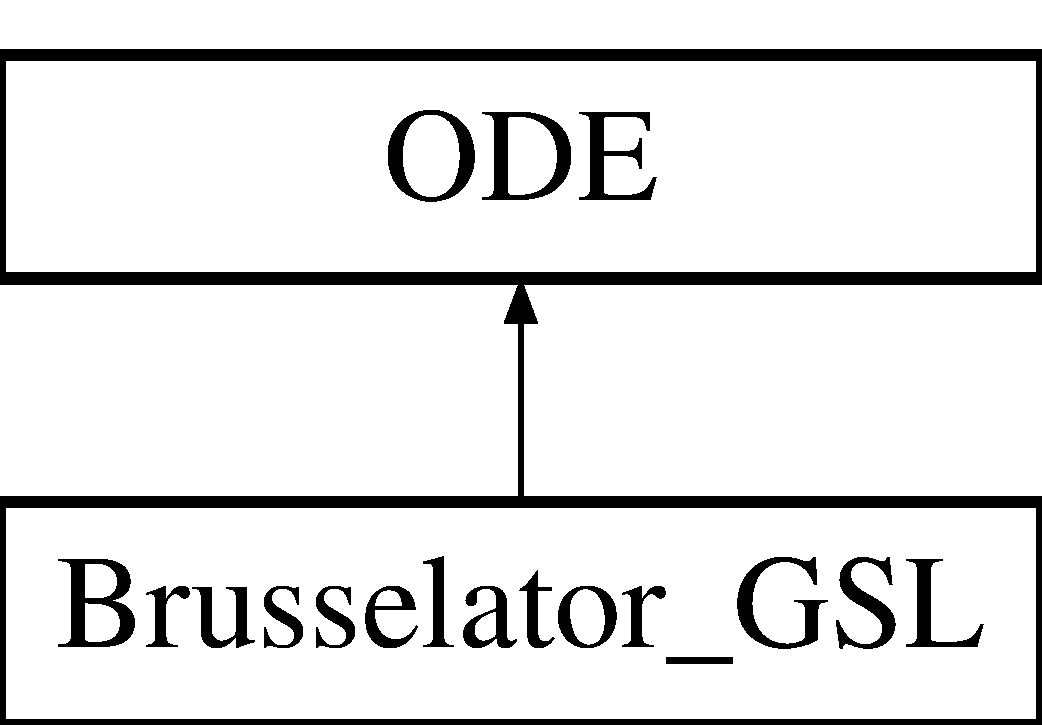
\includegraphics[height=2.000000cm]{classBrusselator__GSL}
\end{center}
\end{figure}
\subsubsection*{Public Member Functions}
\begin{DoxyCompactItemize}
\item 
{\bf Brusselator\+\_\+\+G\+S\+L} (int my\+\_\+neq, int my\+\_\+nt, double my\+\_\+ti, double my\+\_\+tf, double my\+\_\+dt)
\item 
void {\bf rhs} (double t, double $\ast$u, double $\ast$f)
\item 
void {\bf step} (double t, double $\ast$u, double $\ast$unew)
\end{DoxyCompactItemize}
\subsubsection*{Data Fields}
\begin{DoxyCompactItemize}
\item 
int {\bf neq}
\item 
int {\bf nt}
\item 
double {\bf ti}
\item 
double {\bf tf}
\item 
double {\bf dt}
\end{DoxyCompactItemize}
\subsubsection*{Private Member Functions}
\begin{DoxyCompactItemize}
\item 
void {\bf newt} (double t, double $\ast$uprev, double $\ast$uguess, double $\ast$g)
\item 
void {\bf jac} (double t, double $\ast$u, double $\ast$J)
\end{DoxyCompactItemize}


\subsubsection{Detailed Description}


Definition at line 10 of file brusselator.\+h.



\subsubsection{Constructor \& Destructor Documentation}
\index{Brusselator\+\_\+\+G\+S\+L@{Brusselator\+\_\+\+G\+S\+L}!Brusselator\+\_\+\+G\+S\+L@{Brusselator\+\_\+\+G\+S\+L}}
\index{Brusselator\+\_\+\+G\+S\+L@{Brusselator\+\_\+\+G\+S\+L}!Brusselator\+\_\+\+G\+S\+L@{Brusselator\+\_\+\+G\+S\+L}}
\paragraph[{Brusselator\+\_\+\+G\+S\+L(int my\+\_\+neq, int my\+\_\+nt, double my\+\_\+ti, double my\+\_\+tf, double my\+\_\+dt)}]{\setlength{\rightskip}{0pt plus 5cm}Brusselator\+\_\+\+G\+S\+L\+::\+Brusselator\+\_\+\+G\+S\+L (
\begin{DoxyParamCaption}
\item[{int}]{my\+\_\+neq, }
\item[{int}]{my\+\_\+nt, }
\item[{double}]{my\+\_\+ti, }
\item[{double}]{my\+\_\+tf, }
\item[{double}]{my\+\_\+dt}
\end{DoxyParamCaption}
)\hspace{0.3cm}{\ttfamily [inline]}}\label{classBrusselator__GSL_a8479c3c3837aa34e6d8a44e40305b0e6}


Definition at line 12 of file brusselator.\+h.



References O\+D\+E\+::dt, O\+D\+E\+::neq, O\+D\+E\+::nt, O\+D\+E\+::tf, and O\+D\+E\+::ti.



\subsubsection{Member Function Documentation}
\index{Brusselator\+\_\+\+G\+S\+L@{Brusselator\+\_\+\+G\+S\+L}!jac@{jac}}
\index{jac@{jac}!Brusselator\+\_\+\+G\+S\+L@{Brusselator\+\_\+\+G\+S\+L}}
\paragraph[{jac(double t, double $\ast$u, double $\ast$\+J)}]{\setlength{\rightskip}{0pt plus 5cm}void Brusselator\+\_\+\+G\+S\+L\+::jac (
\begin{DoxyParamCaption}
\item[{double}]{t, }
\item[{double $\ast$}]{u, }
\item[{double $\ast$}]{J}
\end{DoxyParamCaption}
)\hspace{0.3cm}{\ttfamily [inline]}, {\ttfamily [private]}}\label{classBrusselator__GSL_ae44dc7d932b081c1a06359aab206dfb7}
Helper function to the Jacobian matrix (using finite differences) for advancing the solution from time t(n) to t(n+1) using an implicit Euler step on a system of equations

\begin{DoxyReturn}{Returns}
(by reference) J the Jacobian for the Newton step 
\end{DoxyReturn}

\begin{DoxyParams}{Parameters}
{\em t} & current time step \\
\hline
{\em u} & function value at the current time step \\
\hline
{\em J} & Jacobian, returned by reference\\
\hline
\end{DoxyParams}


Definition at line 155 of file brusselator.\+h.



References O\+D\+E\+::dt, O\+D\+E\+::neq, and rhs().



Referenced by step().

\index{Brusselator\+\_\+\+G\+S\+L@{Brusselator\+\_\+\+G\+S\+L}!newt@{newt}}
\index{newt@{newt}!Brusselator\+\_\+\+G\+S\+L@{Brusselator\+\_\+\+G\+S\+L}}
\paragraph[{newt(double t, double $\ast$uprev, double $\ast$uguess, double $\ast$g)}]{\setlength{\rightskip}{0pt plus 5cm}void Brusselator\+\_\+\+G\+S\+L\+::newt (
\begin{DoxyParamCaption}
\item[{double}]{t, }
\item[{double $\ast$}]{uprev, }
\item[{double $\ast$}]{uguess, }
\item[{double $\ast$}]{g}
\end{DoxyParamCaption}
)\hspace{0.3cm}{\ttfamily [inline]}, {\ttfamily [private]}}\label{classBrusselator__GSL_adfbabbb536eec4c8c7c8ea0e6e04b84f}
Helper function to compute the next Newton step for solving a system of equations

\begin{DoxyReturn}{Returns}
(by reference) g how far from zero we are 
\end{DoxyReturn}

\begin{DoxyParams}{Parameters}
{\em t} & current time step \\
\hline
{\em uguess} & current solution guess \\
\hline
{\em uprev} & solution at previous time step \\
\hline
{\em g} & how far from zero we are, returned by reference\\
\hline
\end{DoxyParams}


Definition at line 138 of file brusselator.\+h.



References O\+D\+E\+::dt, O\+D\+E\+::neq, and rhs().



Referenced by step().

\index{Brusselator\+\_\+\+G\+S\+L@{Brusselator\+\_\+\+G\+S\+L}!rhs@{rhs}}
\index{rhs@{rhs}!Brusselator\+\_\+\+G\+S\+L@{Brusselator\+\_\+\+G\+S\+L}}
\paragraph[{rhs(double t, double $\ast$u, double $\ast$f)}]{\setlength{\rightskip}{0pt plus 5cm}void Brusselator\+\_\+\+G\+S\+L\+::rhs (
\begin{DoxyParamCaption}
\item[{double}]{t, }
\item[{double $\ast$}]{u, }
\item[{double $\ast$}]{f}
\end{DoxyParamCaption}
)\hspace{0.3cm}{\ttfamily [inline]}, {\ttfamily [virtual]}}\label{classBrusselator__GSL_abee5887ab8e67d01da6bc4ff646dd572}
user implemented rhs function, u\textquotesingle{}=rhs(t,u) \begin{DoxyReturn}{Returns}
(by reference) f\+: rhs(t,u) 
\end{DoxyReturn}

\begin{DoxyParams}{Parameters}
{\em t} & current time step \\
\hline
{\em u} & solution u at time t \\
\hline
{\em f} & rhs(t,u) \\
\hline
\end{DoxyParams}
user implemented rhs function, u\textquotesingle{}=rhs(t,u) \begin{DoxyReturn}{Returns}
(by reference) f\+: rhs(t,u) 
\end{DoxyReturn}

\begin{DoxyParams}{Parameters}
{\em t} & current time step \\
\hline
{\em u} & solution u at time t \\
\hline
{\em f} & rhs(t,u)\\
\hline
\end{DoxyParams}


Implements {\bf O\+D\+E} \doxyref{}{p.}{classODE_a9499def749f2914a41b4616f879c991b}.



Definition at line 20 of file brusselator.\+h.



References O\+D\+E\+::neq.



Referenced by jac(), and newt().

\index{Brusselator\+\_\+\+G\+S\+L@{Brusselator\+\_\+\+G\+S\+L}!step@{step}}
\index{step@{step}!Brusselator\+\_\+\+G\+S\+L@{Brusselator\+\_\+\+G\+S\+L}}
\paragraph[{step(double t, double $\ast$u, double $\ast$unew)}]{\setlength{\rightskip}{0pt plus 5cm}void Brusselator\+\_\+\+G\+S\+L\+::step (
\begin{DoxyParamCaption}
\item[{double}]{t, }
\item[{double $\ast$}]{u, }
\item[{double $\ast$}]{unew}
\end{DoxyParamCaption}
)\hspace{0.3cm}{\ttfamily [inline]}, {\ttfamily [virtual]}}\label{classBrusselator__GSL_a8ed20dea95f4b1705030f0aeee2deacb}
user implemented step function, for advancing the solution from t to t+dt \begin{DoxyReturn}{Returns}
(by reference) unew\+: solution at time t+dt 
\end{DoxyReturn}

\begin{DoxyParams}{Parameters}
{\em t} & current time step \\
\hline
{\em u} & solution u at time t \\
\hline
{\em unew} & solution at time t+dt \\
\hline
\end{DoxyParams}
user implemented step function, for advancing the solution from t to t+dt \begin{DoxyReturn}{Returns}
(by reference) unew\+: solution at time t+dt 
\end{DoxyReturn}

\begin{DoxyParams}{Parameters}
{\em t} & current time step \\
\hline
{\em u} & solution u at time t \\
\hline
{\em unew} & solution at time t+dt\\
\hline
\end{DoxyParams}


Implements {\bf O\+D\+E} \doxyref{}{p.}{classODE_a966f35008ac30511d950b557f53b7468}.



Definition at line 47 of file brusselator.\+h.



References O\+D\+E\+::dt, jac(), O\+D\+E\+::neq, and newt().



\subsubsection{Field Documentation}
\index{Brusselator\+\_\+\+G\+S\+L@{Brusselator\+\_\+\+G\+S\+L}!dt@{dt}}
\index{dt@{dt}!Brusselator\+\_\+\+G\+S\+L@{Brusselator\+\_\+\+G\+S\+L}}
\paragraph[{dt}]{\setlength{\rightskip}{0pt plus 5cm}double O\+D\+E\+::dt\hspace{0.3cm}{\ttfamily [inherited]}}\label{classODE_a489591849cd00a583407cde072b51acd}
time step 

Definition at line 33 of file ridc.\+h.



Referenced by Brusselator\+\_\+\+G\+S\+L(), corr\+\_\+be(), corr\+\_\+fe(), jac(), newt(), ridc\+\_\+be(), ridc\+\_\+fe(), and step().

\index{Brusselator\+\_\+\+G\+S\+L@{Brusselator\+\_\+\+G\+S\+L}!neq@{neq}}
\index{neq@{neq}!Brusselator\+\_\+\+G\+S\+L@{Brusselator\+\_\+\+G\+S\+L}}
\paragraph[{neq}]{\setlength{\rightskip}{0pt plus 5cm}int O\+D\+E\+::neq\hspace{0.3cm}{\ttfamily [inherited]}}\label{classODE_ad10440423b2185d322223da17d1135c5}
number of equations 

Definition at line 21 of file ridc.\+h.



Referenced by Brusselator\+\_\+\+G\+S\+L(), corr\+\_\+be(), corr\+\_\+fe(), jac(), newt(), rhs(), ridc\+\_\+be(), ridc\+\_\+fe(), and step().

\index{Brusselator\+\_\+\+G\+S\+L@{Brusselator\+\_\+\+G\+S\+L}!nt@{nt}}
\index{nt@{nt}!Brusselator\+\_\+\+G\+S\+L@{Brusselator\+\_\+\+G\+S\+L}}
\paragraph[{nt}]{\setlength{\rightskip}{0pt plus 5cm}int O\+D\+E\+::nt\hspace{0.3cm}{\ttfamily [inherited]}}\label{classODE_a275faaf08a8602b6a0c60131d3b874b0}
number of time steps 

Definition at line 24 of file ridc.\+h.



Referenced by Brusselator\+\_\+\+G\+S\+L(), ridc\+\_\+be(), and ridc\+\_\+fe().

\index{Brusselator\+\_\+\+G\+S\+L@{Brusselator\+\_\+\+G\+S\+L}!tf@{tf}}
\index{tf@{tf}!Brusselator\+\_\+\+G\+S\+L@{Brusselator\+\_\+\+G\+S\+L}}
\paragraph[{tf}]{\setlength{\rightskip}{0pt plus 5cm}double O\+D\+E\+::tf\hspace{0.3cm}{\ttfamily [inherited]}}\label{classODE_aa53beae63fb47d22abca58dd4a407e9e}
final time 

Definition at line 30 of file ridc.\+h.



Referenced by Brusselator\+\_\+\+G\+S\+L().

\index{Brusselator\+\_\+\+G\+S\+L@{Brusselator\+\_\+\+G\+S\+L}!ti@{ti}}
\index{ti@{ti}!Brusselator\+\_\+\+G\+S\+L@{Brusselator\+\_\+\+G\+S\+L}}
\paragraph[{ti}]{\setlength{\rightskip}{0pt plus 5cm}double O\+D\+E\+::ti\hspace{0.3cm}{\ttfamily [inherited]}}\label{classODE_abaa6d4b370ec903c7a1f53de5d758cf1}
initial time 

Definition at line 27 of file ridc.\+h.



Referenced by Brusselator\+\_\+\+G\+S\+L(), ridc\+\_\+be(), and ridc\+\_\+fe().



The documentation for this class was generated from the following file\+:\begin{DoxyCompactItemize}
\item 
examples/brusselator\+\_\+gsl/{\bf brusselator.\+h}\end{DoxyCompactItemize}

\subsection{Brusselator\+\_\+\+M\+K\+L Class Reference}
\label{classBrusselator__MKL}\index{Brusselator\+\_\+\+M\+K\+L@{Brusselator\+\_\+\+M\+K\+L}}


{\ttfamily \#include $<$brusselator.\+h$>$}

Inheritance diagram for Brusselator\+\_\+\+M\+K\+L\+:\begin{figure}[H]
\begin{center}
\leavevmode
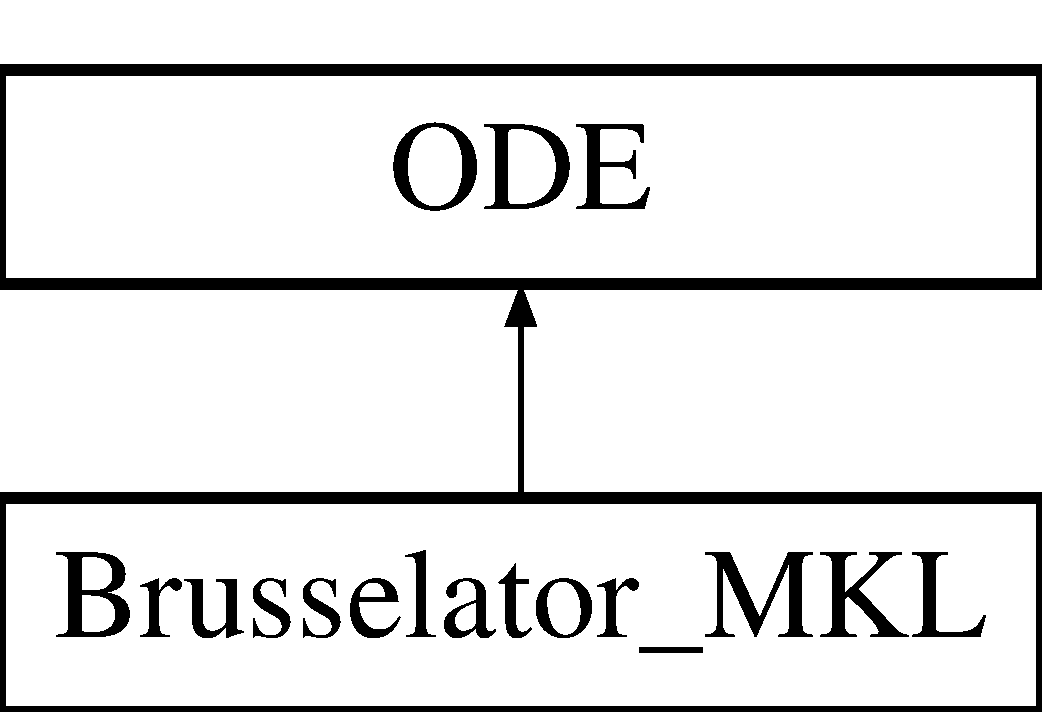
\includegraphics[height=2.000000cm]{classBrusselator__MKL}
\end{center}
\end{figure}
\subsubsection*{Public Member Functions}
\begin{DoxyCompactItemize}
\item 
{\bf Brusselator\+\_\+\+M\+K\+L} (int my\+\_\+neq, int my\+\_\+nt, double my\+\_\+ti, double my\+\_\+tf, double my\+\_\+dt)
\item 
void {\bf rhs} (double t, double $\ast$u, double $\ast$f)
\item 
void {\bf step} (double t, double $\ast$u, double $\ast$unew)
\end{DoxyCompactItemize}
\subsubsection*{Data Fields}
\begin{DoxyCompactItemize}
\item 
int {\bf neq}
\item 
int {\bf nt}
\item 
double {\bf ti}
\item 
double {\bf tf}
\item 
double {\bf dt}
\end{DoxyCompactItemize}
\subsubsection*{Private Member Functions}
\begin{DoxyCompactItemize}
\item 
void {\bf newt} (double t, double $\ast$uprev, double $\ast$uguess, double $\ast$g)
\item 
void {\bf jac} (double t, double $\ast$u, double $\ast$J)
\end{DoxyCompactItemize}


\subsubsection{Detailed Description}


Definition at line 11 of file brusselator.\+h.



\subsubsection{Constructor \& Destructor Documentation}
\index{Brusselator\+\_\+\+M\+K\+L@{Brusselator\+\_\+\+M\+K\+L}!Brusselator\+\_\+\+M\+K\+L@{Brusselator\+\_\+\+M\+K\+L}}
\index{Brusselator\+\_\+\+M\+K\+L@{Brusselator\+\_\+\+M\+K\+L}!Brusselator\+\_\+\+M\+K\+L@{Brusselator\+\_\+\+M\+K\+L}}
\paragraph[{Brusselator\+\_\+\+M\+K\+L(int my\+\_\+neq, int my\+\_\+nt, double my\+\_\+ti, double my\+\_\+tf, double my\+\_\+dt)}]{\setlength{\rightskip}{0pt plus 5cm}Brusselator\+\_\+\+M\+K\+L\+::\+Brusselator\+\_\+\+M\+K\+L (
\begin{DoxyParamCaption}
\item[{int}]{my\+\_\+neq, }
\item[{int}]{my\+\_\+nt, }
\item[{double}]{my\+\_\+ti, }
\item[{double}]{my\+\_\+tf, }
\item[{double}]{my\+\_\+dt}
\end{DoxyParamCaption}
)\hspace{0.3cm}{\ttfamily [inline]}}\label{classBrusselator__MKL_a356b6fb1a3a2a6f9e79795b1834b3c71}


Definition at line 13 of file brusselator.\+h.



\subsubsection{Member Function Documentation}
\index{Brusselator\+\_\+\+M\+K\+L@{Brusselator\+\_\+\+M\+K\+L}!jac@{jac}}
\index{jac@{jac}!Brusselator\+\_\+\+M\+K\+L@{Brusselator\+\_\+\+M\+K\+L}}
\paragraph[{jac(double t, double $\ast$u, double $\ast$\+J)}]{\setlength{\rightskip}{0pt plus 5cm}void Brusselator\+\_\+\+M\+K\+L\+::jac (
\begin{DoxyParamCaption}
\item[{double}]{t, }
\item[{double $\ast$}]{u, }
\item[{double $\ast$}]{J}
\end{DoxyParamCaption}
)\hspace{0.3cm}{\ttfamily [inline]}, {\ttfamily [private]}}\label{classBrusselator__MKL_ace16b06feefec053278637a23cb94bad}
Helper function to compute the Jacobian matrix (using finite differences) for advancing the solution from time t(n) to t(n+1) using an implicit Euler step on a system of equations

\begin{DoxyReturn}{Returns}
(by reference) J the Jacobian for the Newton step 
\end{DoxyReturn}

\begin{DoxyParams}{Parameters}
{\em t} & current time step \\
\hline
{\em u} & solution value at the current iterate \\
\hline
{\em J} & Jacobian, returned by reference\\
\hline
\end{DoxyParams}


Definition at line 141 of file brusselator.\+h.



References rhs().

\index{Brusselator\+\_\+\+M\+K\+L@{Brusselator\+\_\+\+M\+K\+L}!newt@{newt}}
\index{newt@{newt}!Brusselator\+\_\+\+M\+K\+L@{Brusselator\+\_\+\+M\+K\+L}}
\paragraph[{newt(double t, double $\ast$uprev, double $\ast$uguess, double $\ast$g)}]{\setlength{\rightskip}{0pt plus 5cm}void Brusselator\+\_\+\+M\+K\+L\+::newt (
\begin{DoxyParamCaption}
\item[{double}]{t, }
\item[{double $\ast$}]{uprev, }
\item[{double $\ast$}]{uguess, }
\item[{double $\ast$}]{g}
\end{DoxyParamCaption}
)\hspace{0.3cm}{\ttfamily [inline]}, {\ttfamily [private]}}\label{classBrusselator__MKL_ab4859e93248da4c28f7d06aa4562675c}
Helper function for computing the next Newton step

\begin{DoxyReturn}{Returns}
(by reference) g distance from the root 
\end{DoxyReturn}

\begin{DoxyParams}{Parameters}
{\em t} & current time step \\
\hline
{\em uguess} & current solution guess \\
\hline
{\em uprev} & solution at previous time step \\
\hline
{\em g} & distance from the root, returned by reference\\
\hline
\end{DoxyParams}


Definition at line 125 of file brusselator.\+h.



References rhs().

\index{Brusselator\+\_\+\+M\+K\+L@{Brusselator\+\_\+\+M\+K\+L}!rhs@{rhs}}
\index{rhs@{rhs}!Brusselator\+\_\+\+M\+K\+L@{Brusselator\+\_\+\+M\+K\+L}}
\paragraph[{rhs(double t, double $\ast$u, double $\ast$f)}]{\setlength{\rightskip}{0pt plus 5cm}void Brusselator\+\_\+\+M\+K\+L\+::rhs (
\begin{DoxyParamCaption}
\item[{double}]{t, }
\item[{double $\ast$}]{u, }
\item[{double $\ast$}]{f}
\end{DoxyParamCaption}
)\hspace{0.3cm}{\ttfamily [inline]}, {\ttfamily [virtual]}}\label{classBrusselator__MKL_a90e55526052241ef810c61cf7ebf382f}
user implemented rhs function, u\textquotesingle{}=rhs(t,u) \begin{DoxyReturn}{Returns}
(by reference) f\+: rhs(t,u) 
\end{DoxyReturn}

\begin{DoxyParams}{Parameters}
{\em t} & current time step \\
\hline
{\em u} & solution u at time t \\
\hline
{\em f} & rhs(t,u) \\
\hline
\end{DoxyParams}
user implemented rhs function, u\textquotesingle{}=rhs(t,u) \begin{DoxyReturn}{Returns}
(by reference) f\+: rhs(t,u) 
\end{DoxyReturn}

\begin{DoxyParams}{Parameters}
{\em t} & current time step \\
\hline
{\em u} & solution u at time t \\
\hline
{\em f} & rhs(t,u)\\
\hline
\end{DoxyParams}


Implements {\bf O\+D\+E} \doxyref{}{p.}{classODE_a9499def749f2914a41b4616f879c991b}.



Definition at line 21 of file brusselator.\+h.

\index{Brusselator\+\_\+\+M\+K\+L@{Brusselator\+\_\+\+M\+K\+L}!step@{step}}
\index{step@{step}!Brusselator\+\_\+\+M\+K\+L@{Brusselator\+\_\+\+M\+K\+L}}
\paragraph[{step(double t, double $\ast$u, double $\ast$unew)}]{\setlength{\rightskip}{0pt plus 5cm}void Brusselator\+\_\+\+M\+K\+L\+::step (
\begin{DoxyParamCaption}
\item[{double}]{t, }
\item[{double $\ast$}]{u, }
\item[{double $\ast$}]{unew}
\end{DoxyParamCaption}
)\hspace{0.3cm}{\ttfamily [inline]}, {\ttfamily [virtual]}}\label{classBrusselator__MKL_a3193b7fb7ec213ebd468eafa1e66c020}
user implemented step function, for advancing the solution from t to t+dt \begin{DoxyReturn}{Returns}
(by reference) unew\+: solution at time t+dt 
\end{DoxyReturn}

\begin{DoxyParams}{Parameters}
{\em t} & current time step \\
\hline
{\em u} & solution u at time t \\
\hline
{\em unew} & solution at time t+dt \\
\hline
\end{DoxyParams}
user implemented step function, for advancing the solution from t to t+dt \begin{DoxyReturn}{Returns}
(by reference) unew\+: solution at time t+dt 
\end{DoxyReturn}

\begin{DoxyParams}{Parameters}
{\em t} & current time step \\
\hline
{\em u} & solution u at time t \\
\hline
{\em unew} & solution at time t+dt\\
\hline
\end{DoxyParams}


Implements {\bf O\+D\+E} \doxyref{}{p.}{classODE_a966f35008ac30511d950b557f53b7468}.



Definition at line 48 of file brusselator.\+h.



References jac(), and newt().



\subsubsection{Field Documentation}
\index{Brusselator\+\_\+\+M\+K\+L@{Brusselator\+\_\+\+M\+K\+L}!dt@{dt}}
\index{dt@{dt}!Brusselator\+\_\+\+M\+K\+L@{Brusselator\+\_\+\+M\+K\+L}}
\paragraph[{dt}]{\setlength{\rightskip}{0pt plus 5cm}double O\+D\+E\+::dt\hspace{0.3cm}{\ttfamily [inherited]}}\label{classODE_a489591849cd00a583407cde072b51acd}
time step 

Definition at line 33 of file ridc.\+h.



Referenced by Brusselator\+\_\+\+G\+S\+L\+::\+Brusselator\+\_\+\+G\+S\+L(), corr\+\_\+be(), corr\+\_\+fe(), Brusselator\+\_\+\+G\+S\+L\+::jac(), Brusselator\+\_\+\+G\+S\+L\+::newt(), ridc\+\_\+be(), ridc\+\_\+fe(), and Brusselator\+\_\+\+G\+S\+L\+::step().

\index{Brusselator\+\_\+\+M\+K\+L@{Brusselator\+\_\+\+M\+K\+L}!neq@{neq}}
\index{neq@{neq}!Brusselator\+\_\+\+M\+K\+L@{Brusselator\+\_\+\+M\+K\+L}}
\paragraph[{neq}]{\setlength{\rightskip}{0pt plus 5cm}int O\+D\+E\+::neq\hspace{0.3cm}{\ttfamily [inherited]}}\label{classODE_ad10440423b2185d322223da17d1135c5}
number of equations 

Definition at line 21 of file ridc.\+h.



Referenced by Brusselator\+\_\+\+G\+S\+L\+::\+Brusselator\+\_\+\+G\+S\+L(), corr\+\_\+be(), corr\+\_\+fe(), Brusselator\+\_\+\+G\+S\+L\+::jac(), Brusselator\+\_\+\+G\+S\+L\+::newt(), Brusselator\+\_\+\+G\+S\+L\+::rhs(), ridc\+\_\+be(), ridc\+\_\+fe(), and Brusselator\+\_\+\+G\+S\+L\+::step().

\index{Brusselator\+\_\+\+M\+K\+L@{Brusselator\+\_\+\+M\+K\+L}!nt@{nt}}
\index{nt@{nt}!Brusselator\+\_\+\+M\+K\+L@{Brusselator\+\_\+\+M\+K\+L}}
\paragraph[{nt}]{\setlength{\rightskip}{0pt plus 5cm}int O\+D\+E\+::nt\hspace{0.3cm}{\ttfamily [inherited]}}\label{classODE_a275faaf08a8602b6a0c60131d3b874b0}
number of time steps 

Definition at line 24 of file ridc.\+h.



Referenced by Brusselator\+\_\+\+G\+S\+L\+::\+Brusselator\+\_\+\+G\+S\+L(), ridc\+\_\+be(), and ridc\+\_\+fe().

\index{Brusselator\+\_\+\+M\+K\+L@{Brusselator\+\_\+\+M\+K\+L}!tf@{tf}}
\index{tf@{tf}!Brusselator\+\_\+\+M\+K\+L@{Brusselator\+\_\+\+M\+K\+L}}
\paragraph[{tf}]{\setlength{\rightskip}{0pt plus 5cm}double O\+D\+E\+::tf\hspace{0.3cm}{\ttfamily [inherited]}}\label{classODE_aa53beae63fb47d22abca58dd4a407e9e}
final time 

Definition at line 30 of file ridc.\+h.



Referenced by Brusselator\+\_\+\+G\+S\+L\+::\+Brusselator\+\_\+\+G\+S\+L().

\index{Brusselator\+\_\+\+M\+K\+L@{Brusselator\+\_\+\+M\+K\+L}!ti@{ti}}
\index{ti@{ti}!Brusselator\+\_\+\+M\+K\+L@{Brusselator\+\_\+\+M\+K\+L}}
\paragraph[{ti}]{\setlength{\rightskip}{0pt plus 5cm}double O\+D\+E\+::ti\hspace{0.3cm}{\ttfamily [inherited]}}\label{classODE_abaa6d4b370ec903c7a1f53de5d758cf1}
initial time 

Definition at line 27 of file ridc.\+h.



Referenced by Brusselator\+\_\+\+G\+S\+L\+::\+Brusselator\+\_\+\+G\+S\+L(), ridc\+\_\+be(), and ridc\+\_\+fe().



The documentation for this class was generated from the following file\+:\begin{DoxyCompactItemize}
\item 
examples/brusselator\+\_\+mkl/{\bf brusselator.\+h}\end{DoxyCompactItemize}

\subsection{B\+U\+T\+C\+H\+E\+R Struct Reference}
\label{structBUTCHER}\index{B\+U\+T\+C\+H\+E\+R@{B\+U\+T\+C\+H\+E\+R}}


{\ttfamily \#include $<$ode.\+h$>$}

\subsubsection*{Data Fields}
\begin{DoxyCompactItemize}
\item 
int {\bf S}
\item 
double $\ast$ {\bf b}
\item 
double $\ast$ {\bf c}
\item 
double $\ast$$\ast$ {\bf A}
\end{DoxyCompactItemize}


\subsubsection{Detailed Description}


Definition at line 21 of file ode.\+h.



\subsubsection{Field Documentation}
\index{B\+U\+T\+C\+H\+E\+R@{B\+U\+T\+C\+H\+E\+R}!A@{A}}
\index{A@{A}!B\+U\+T\+C\+H\+E\+R@{B\+U\+T\+C\+H\+E\+R}}
\paragraph[{A}]{\setlength{\rightskip}{0pt plus 5cm}double$\ast$$\ast$ B\+U\+T\+C\+H\+E\+R\+::\+A}\label{structBUTCHER_a4b7de674ab073c62428dffd65f15a0d2}


Definition at line 25 of file ode.\+h.



Referenced by main(), and newt().

\index{B\+U\+T\+C\+H\+E\+R@{B\+U\+T\+C\+H\+E\+R}!b@{b}}
\index{b@{b}!B\+U\+T\+C\+H\+E\+R@{B\+U\+T\+C\+H\+E\+R}}
\paragraph[{b}]{\setlength{\rightskip}{0pt plus 5cm}double$\ast$ B\+U\+T\+C\+H\+E\+R\+::b}\label{structBUTCHER_a294a17cbbdd7e1f33f2fcb7d912c1bb9}


Definition at line 23 of file ode.\+h.



Referenced by main(), and step().

\index{B\+U\+T\+C\+H\+E\+R@{B\+U\+T\+C\+H\+E\+R}!c@{c}}
\index{c@{c}!B\+U\+T\+C\+H\+E\+R@{B\+U\+T\+C\+H\+E\+R}}
\paragraph[{c}]{\setlength{\rightskip}{0pt plus 5cm}double$\ast$ B\+U\+T\+C\+H\+E\+R\+::c}\label{structBUTCHER_a3dc46ec7591b13f9ba6d948e10729d62}


Definition at line 24 of file ode.\+h.



Referenced by main(), newt(), and step().

\index{B\+U\+T\+C\+H\+E\+R@{B\+U\+T\+C\+H\+E\+R}!S@{S}}
\index{S@{S}!B\+U\+T\+C\+H\+E\+R@{B\+U\+T\+C\+H\+E\+R}}
\paragraph[{S}]{\setlength{\rightskip}{0pt plus 5cm}int B\+U\+T\+C\+H\+E\+R\+::\+S}\label{structBUTCHER_a175f670f536987c25dcfdcb0856b1393}


Definition at line 22 of file ode.\+h.



Referenced by jac(), main(), newt(), and step().



The documentation for this struct was generated from the following file\+:\begin{DoxyCompactItemize}
\item 
examples/brusselator\+\_\+radau\+\_\+mkl/{\bf ode.\+h}\end{DoxyCompactItemize}

\subsection{Explicit\+Ode Class Reference}
\label{classExplicitOde}\index{Explicit\+Ode@{Explicit\+Ode}}
Inheritance diagram for Explicit\+Ode\+:\begin{figure}[H]
\begin{center}
\leavevmode
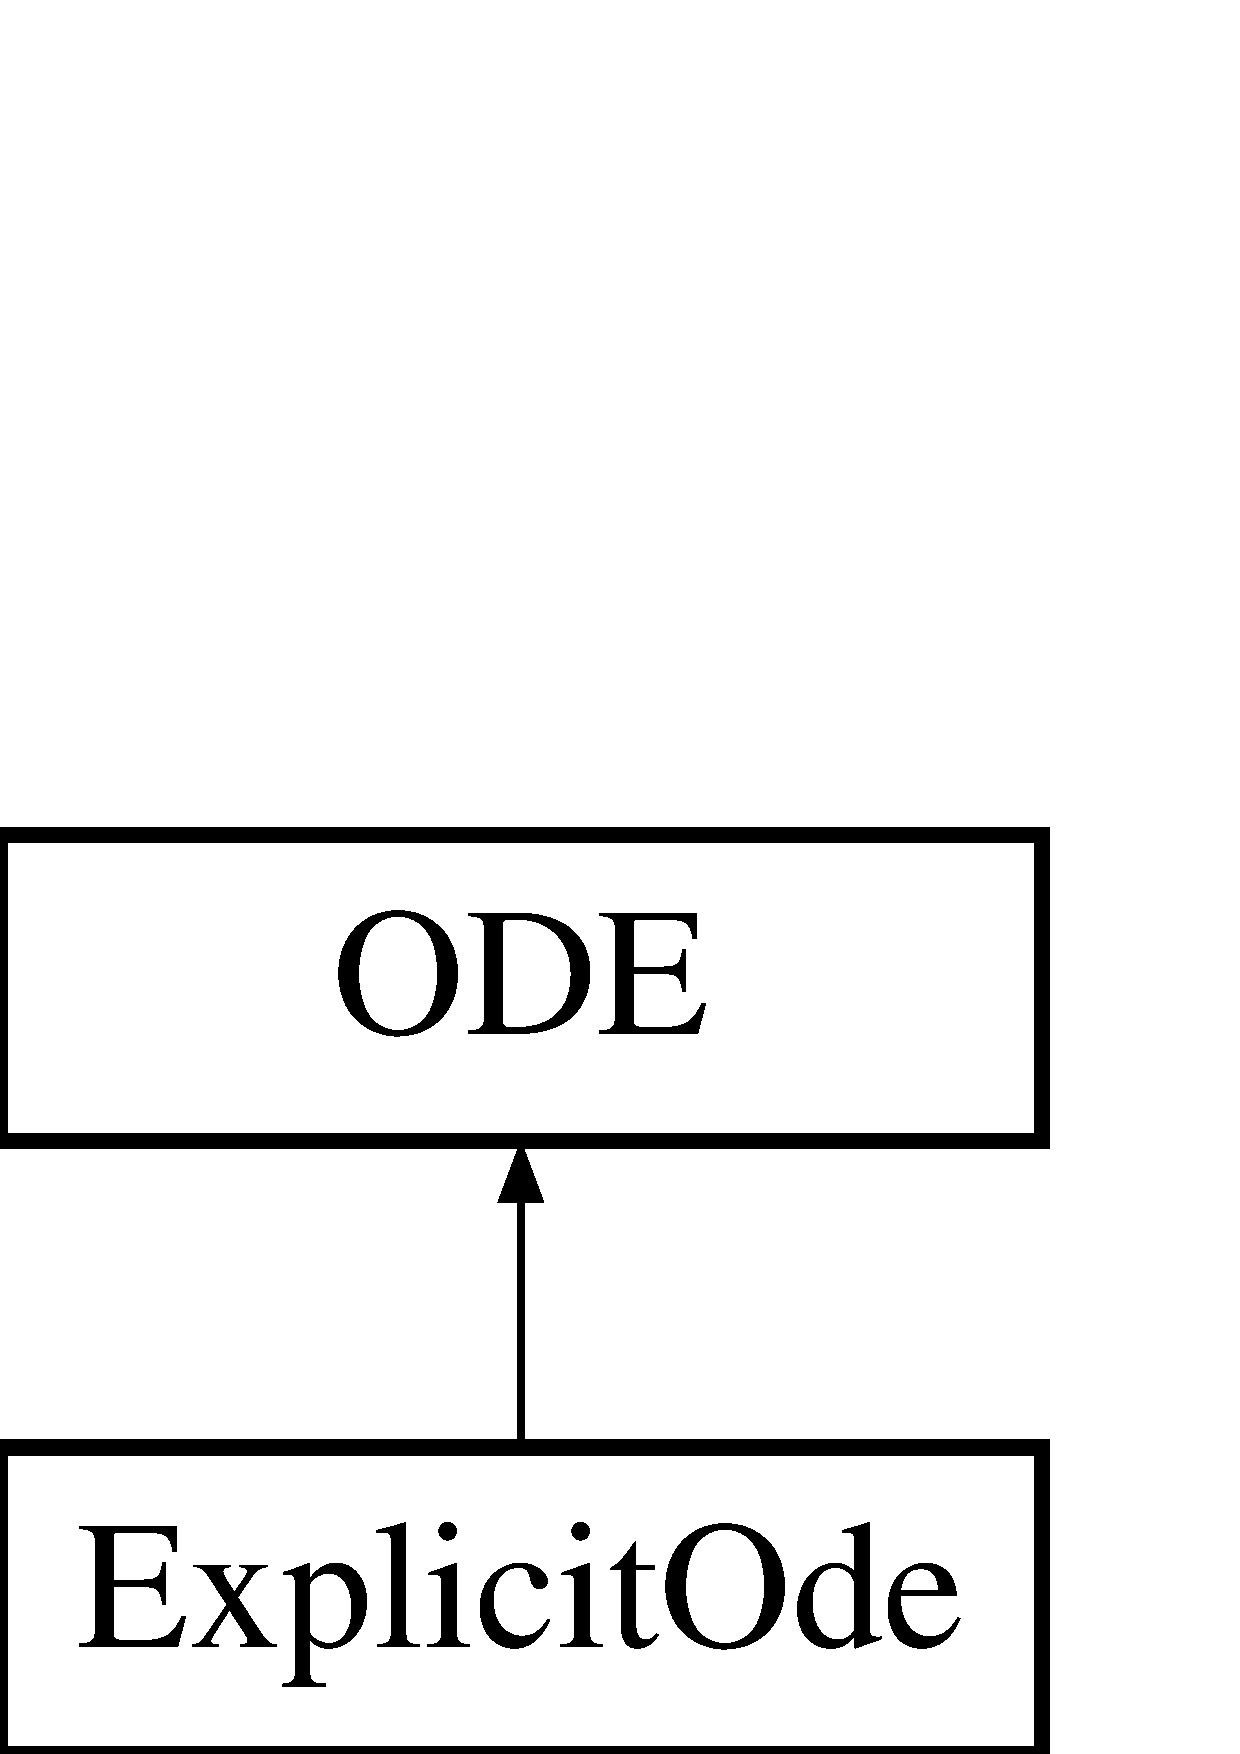
\includegraphics[height=2.000000cm]{classExplicitOde}
\end{center}
\end{figure}
\subsubsection*{Public Member Functions}
\begin{DoxyCompactItemize}
\item 
{\bf Explicit\+Ode} (int my\+\_\+neq, int my\+\_\+nt, double my\+\_\+ti, double my\+\_\+tf, double my\+\_\+dt)
\item 
void {\bf rhs} (double t, double $\ast$u, double $\ast$f)
\item 
void {\bf step} (double t, double $\ast$u, double $\ast$unew)
\end{DoxyCompactItemize}
\subsubsection*{Data Fields}
\begin{DoxyCompactItemize}
\item 
int {\bf neq}
\item 
int {\bf nt}
\item 
double {\bf ti}
\item 
double {\bf tf}
\item 
double {\bf dt}
\end{DoxyCompactItemize}


\subsubsection{Detailed Description}


Definition at line 10 of file explicit.\+cpp.



\subsubsection{Constructor \& Destructor Documentation}
\index{Explicit\+Ode@{Explicit\+Ode}!Explicit\+Ode@{Explicit\+Ode}}
\index{Explicit\+Ode@{Explicit\+Ode}!Explicit\+Ode@{Explicit\+Ode}}
\paragraph[{Explicit\+Ode(int my\+\_\+neq, int my\+\_\+nt, double my\+\_\+ti, double my\+\_\+tf, double my\+\_\+dt)}]{\setlength{\rightskip}{0pt plus 5cm}Explicit\+Ode\+::\+Explicit\+Ode (
\begin{DoxyParamCaption}
\item[{int}]{my\+\_\+neq, }
\item[{int}]{my\+\_\+nt, }
\item[{double}]{my\+\_\+ti, }
\item[{double}]{my\+\_\+tf, }
\item[{double}]{my\+\_\+dt}
\end{DoxyParamCaption}
)\hspace{0.3cm}{\ttfamily [inline]}}\label{classExplicitOde_a706cb79b8b7fc8518d985f670664d1b3}


Definition at line 12 of file explicit.\+cpp.



\subsubsection{Member Function Documentation}
\index{Explicit\+Ode@{Explicit\+Ode}!rhs@{rhs}}
\index{rhs@{rhs}!Explicit\+Ode@{Explicit\+Ode}}
\paragraph[{rhs(double t, double $\ast$u, double $\ast$f)}]{\setlength{\rightskip}{0pt plus 5cm}void Explicit\+Ode\+::rhs (
\begin{DoxyParamCaption}
\item[{double}]{t, }
\item[{double $\ast$}]{u, }
\item[{double $\ast$}]{f}
\end{DoxyParamCaption}
)\hspace{0.3cm}{\ttfamily [inline]}, {\ttfamily [virtual]}}\label{classExplicitOde_a6298c3cda439d026165d08d1c1858ab4}
user implemented rhs function, u\textquotesingle{}=rhs(t,u) \begin{DoxyReturn}{Returns}
(by reference) f\+: rhs(t,u) 
\end{DoxyReturn}

\begin{DoxyParams}{Parameters}
{\em t} & current time step \\
\hline
{\em u} & solution u at time t \\
\hline
{\em f} & rhs(t,u) \\
\hline
\end{DoxyParams}


Implements {\bf O\+D\+E} \doxyref{}{p.}{classODE_a9499def749f2914a41b4616f879c991b}.



Definition at line 20 of file explicit.\+cpp.

\index{Explicit\+Ode@{Explicit\+Ode}!step@{step}}
\index{step@{step}!Explicit\+Ode@{Explicit\+Ode}}
\paragraph[{step(double t, double $\ast$u, double $\ast$unew)}]{\setlength{\rightskip}{0pt plus 5cm}void Explicit\+Ode\+::step (
\begin{DoxyParamCaption}
\item[{double}]{t, }
\item[{double $\ast$}]{u, }
\item[{double $\ast$}]{unew}
\end{DoxyParamCaption}
)\hspace{0.3cm}{\ttfamily [inline]}, {\ttfamily [virtual]}}\label{classExplicitOde_af0d28f83df1cbef1a92433389341597b}
user implemented step function, for advancing the solution from t to t+dt \begin{DoxyReturn}{Returns}
(by reference) unew\+: solution at time t+dt 
\end{DoxyReturn}

\begin{DoxyParams}{Parameters}
{\em t} & current time step \\
\hline
{\em u} & solution u at time t \\
\hline
{\em unew} & solution at time t+dt \\
\hline
\end{DoxyParams}


Implements {\bf O\+D\+E} \doxyref{}{p.}{classODE_a966f35008ac30511d950b557f53b7468}.



Definition at line 26 of file explicit.\+cpp.



References rhs().



\subsubsection{Field Documentation}
\index{Explicit\+Ode@{Explicit\+Ode}!dt@{dt}}
\index{dt@{dt}!Explicit\+Ode@{Explicit\+Ode}}
\paragraph[{dt}]{\setlength{\rightskip}{0pt plus 5cm}double O\+D\+E\+::dt\hspace{0.3cm}{\ttfamily [inherited]}}\label{classODE_a489591849cd00a583407cde072b51acd}
time step 

Definition at line 33 of file ridc.\+h.



Referenced by Brusselator\+\_\+\+G\+S\+L\+::\+Brusselator\+\_\+\+G\+S\+L(), corr\+\_\+be(), corr\+\_\+fe(), Brusselator\+\_\+\+G\+S\+L\+::jac(), Brusselator\+\_\+\+G\+S\+L\+::newt(), ridc\+\_\+be(), ridc\+\_\+fe(), and Brusselator\+\_\+\+G\+S\+L\+::step().

\index{Explicit\+Ode@{Explicit\+Ode}!neq@{neq}}
\index{neq@{neq}!Explicit\+Ode@{Explicit\+Ode}}
\paragraph[{neq}]{\setlength{\rightskip}{0pt plus 5cm}int O\+D\+E\+::neq\hspace{0.3cm}{\ttfamily [inherited]}}\label{classODE_ad10440423b2185d322223da17d1135c5}
number of equations 

Definition at line 21 of file ridc.\+h.



Referenced by Brusselator\+\_\+\+G\+S\+L\+::\+Brusselator\+\_\+\+G\+S\+L(), corr\+\_\+be(), corr\+\_\+fe(), Brusselator\+\_\+\+G\+S\+L\+::jac(), Brusselator\+\_\+\+G\+S\+L\+::newt(), Brusselator\+\_\+\+G\+S\+L\+::rhs(), ridc\+\_\+be(), ridc\+\_\+fe(), and Brusselator\+\_\+\+G\+S\+L\+::step().

\index{Explicit\+Ode@{Explicit\+Ode}!nt@{nt}}
\index{nt@{nt}!Explicit\+Ode@{Explicit\+Ode}}
\paragraph[{nt}]{\setlength{\rightskip}{0pt plus 5cm}int O\+D\+E\+::nt\hspace{0.3cm}{\ttfamily [inherited]}}\label{classODE_a275faaf08a8602b6a0c60131d3b874b0}
number of time steps 

Definition at line 24 of file ridc.\+h.



Referenced by Brusselator\+\_\+\+G\+S\+L\+::\+Brusselator\+\_\+\+G\+S\+L(), ridc\+\_\+be(), and ridc\+\_\+fe().

\index{Explicit\+Ode@{Explicit\+Ode}!tf@{tf}}
\index{tf@{tf}!Explicit\+Ode@{Explicit\+Ode}}
\paragraph[{tf}]{\setlength{\rightskip}{0pt plus 5cm}double O\+D\+E\+::tf\hspace{0.3cm}{\ttfamily [inherited]}}\label{classODE_aa53beae63fb47d22abca58dd4a407e9e}
final time 

Definition at line 30 of file ridc.\+h.



Referenced by Brusselator\+\_\+\+G\+S\+L\+::\+Brusselator\+\_\+\+G\+S\+L().

\index{Explicit\+Ode@{Explicit\+Ode}!ti@{ti}}
\index{ti@{ti}!Explicit\+Ode@{Explicit\+Ode}}
\paragraph[{ti}]{\setlength{\rightskip}{0pt plus 5cm}double O\+D\+E\+::ti\hspace{0.3cm}{\ttfamily [inherited]}}\label{classODE_abaa6d4b370ec903c7a1f53de5d758cf1}
initial time 

Definition at line 27 of file ridc.\+h.



Referenced by Brusselator\+\_\+\+G\+S\+L\+::\+Brusselator\+\_\+\+G\+S\+L(), ridc\+\_\+be(), and ridc\+\_\+fe().



The documentation for this class was generated from the following file\+:\begin{DoxyCompactItemize}
\item 
examples/explicit/{\bf explicit.\+cpp}\end{DoxyCompactItemize}

\subsection{Implicit\+M\+K\+L Class Reference}
\label{classImplicitMKL}\index{Implicit\+M\+K\+L@{Implicit\+M\+K\+L}}


{\ttfamily \#include $<$implicit.\+h$>$}

Inheritance diagram for Implicit\+M\+K\+L\+:\begin{figure}[H]
\begin{center}
\leavevmode
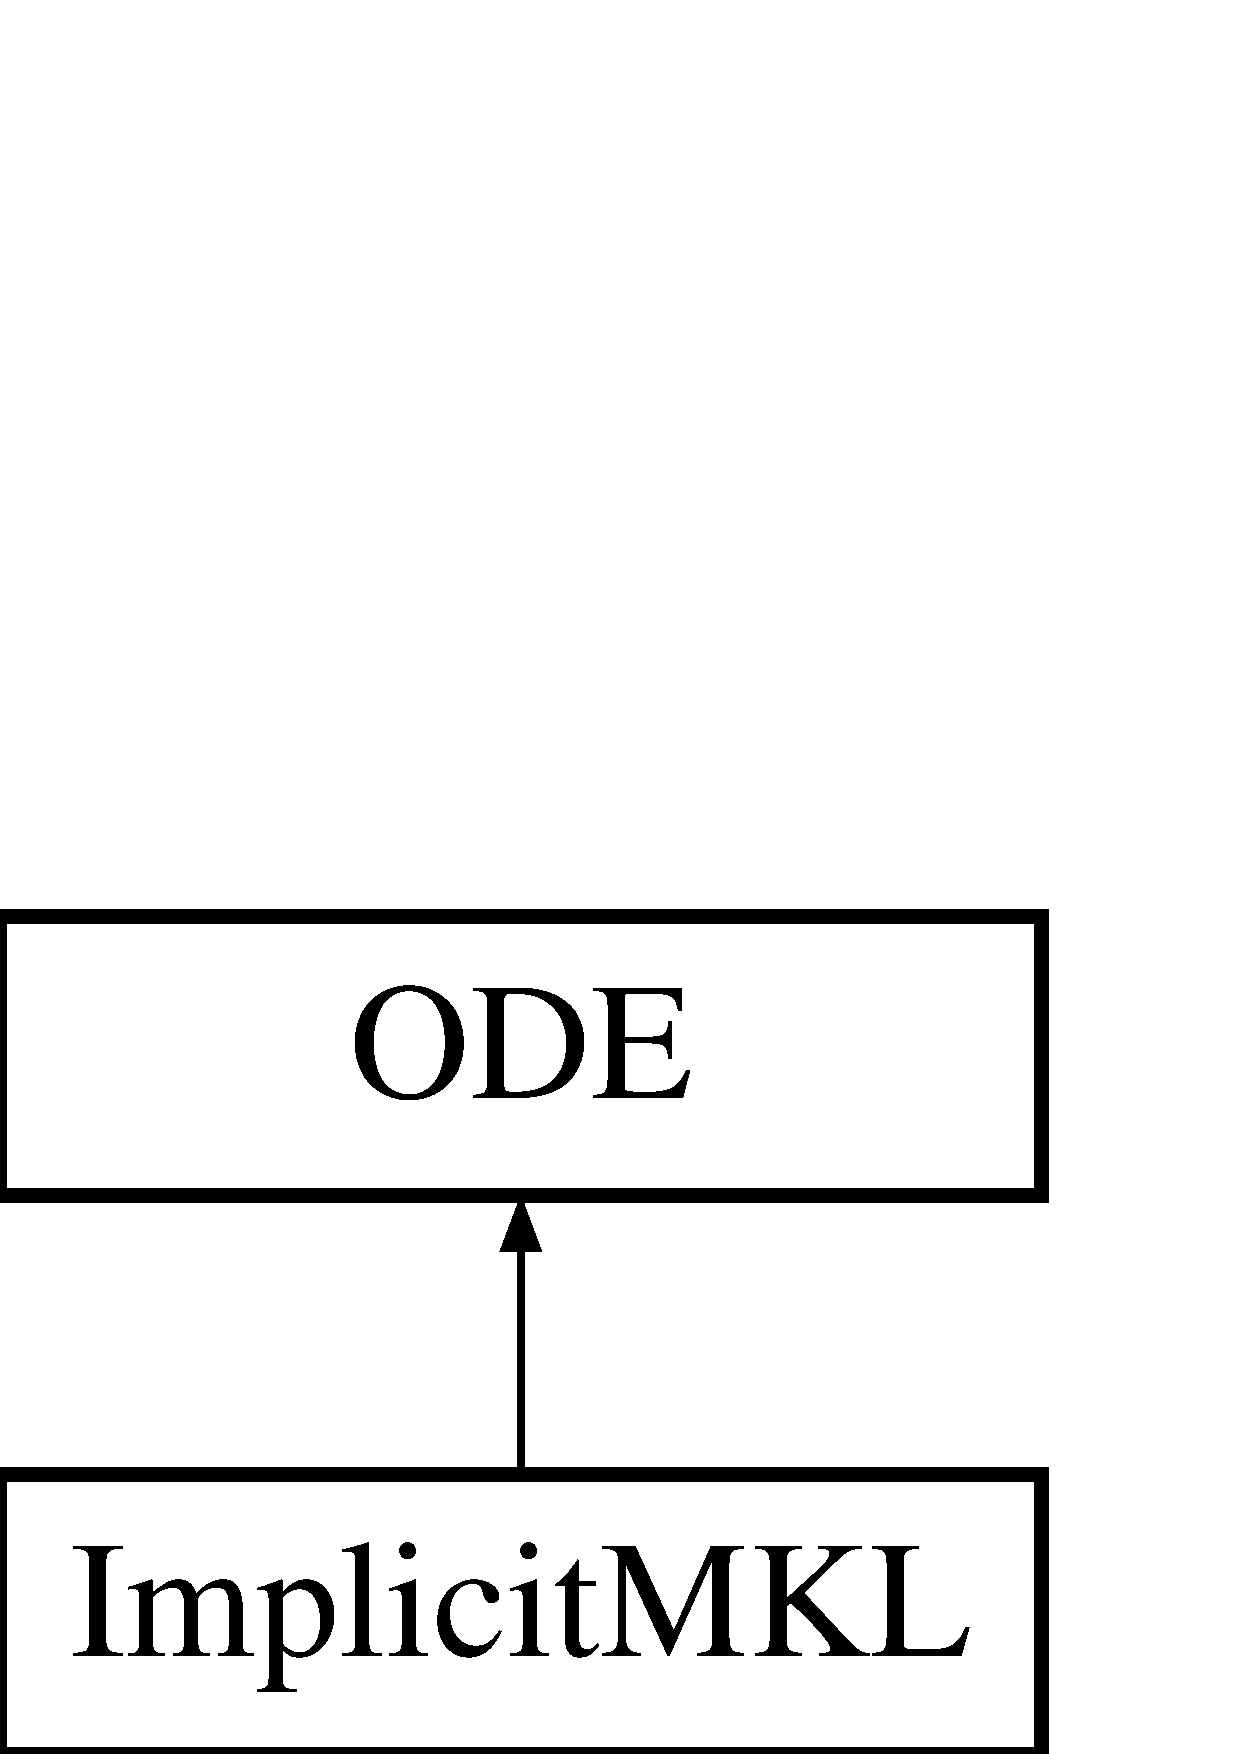
\includegraphics[height=2.000000cm]{classImplicitMKL}
\end{center}
\end{figure}
\subsubsection*{Public Member Functions}
\begin{DoxyCompactItemize}
\item 
{\bf Implicit\+M\+K\+L} (int my\+\_\+neq, int my\+\_\+nt, double my\+\_\+ti, double my\+\_\+tf, double my\+\_\+dt)
\item 
void {\bf rhs} (double t, double $\ast$u, double $\ast$f)
\item 
void {\bf step} (double t, double $\ast$u, double $\ast$unew)
\end{DoxyCompactItemize}
\subsubsection*{Data Fields}
\begin{DoxyCompactItemize}
\item 
int {\bf neq}
\item 
int {\bf nt}
\item 
double {\bf ti}
\item 
double {\bf tf}
\item 
double {\bf dt}
\end{DoxyCompactItemize}
\subsubsection*{Private Member Functions}
\begin{DoxyCompactItemize}
\item 
void {\bf newt} (double t, double $\ast$uprev, double $\ast$uguess, double $\ast$g)
\item 
void {\bf jac} (double t, double $\ast$u, double $\ast$J)
\end{DoxyCompactItemize}


\subsubsection{Detailed Description}


Definition at line 11 of file implicit.\+h.



\subsubsection{Constructor \& Destructor Documentation}
\index{Implicit\+M\+K\+L@{Implicit\+M\+K\+L}!Implicit\+M\+K\+L@{Implicit\+M\+K\+L}}
\index{Implicit\+M\+K\+L@{Implicit\+M\+K\+L}!Implicit\+M\+K\+L@{Implicit\+M\+K\+L}}
\paragraph[{Implicit\+M\+K\+L(int my\+\_\+neq, int my\+\_\+nt, double my\+\_\+ti, double my\+\_\+tf, double my\+\_\+dt)}]{\setlength{\rightskip}{0pt plus 5cm}Implicit\+M\+K\+L\+::\+Implicit\+M\+K\+L (
\begin{DoxyParamCaption}
\item[{int}]{my\+\_\+neq, }
\item[{int}]{my\+\_\+nt, }
\item[{double}]{my\+\_\+ti, }
\item[{double}]{my\+\_\+tf, }
\item[{double}]{my\+\_\+dt}
\end{DoxyParamCaption}
)\hspace{0.3cm}{\ttfamily [inline]}}\label{classImplicitMKL_a787875b2e52713705ba39c56f68f072b}


Definition at line 13 of file implicit.\+h.



\subsubsection{Member Function Documentation}
\index{Implicit\+M\+K\+L@{Implicit\+M\+K\+L}!jac@{jac}}
\index{jac@{jac}!Implicit\+M\+K\+L@{Implicit\+M\+K\+L}}
\paragraph[{jac(double t, double $\ast$u, double $\ast$\+J)}]{\setlength{\rightskip}{0pt plus 5cm}void Implicit\+M\+K\+L\+::jac (
\begin{DoxyParamCaption}
\item[{double}]{t, }
\item[{double $\ast$}]{u, }
\item[{double $\ast$}]{J}
\end{DoxyParamCaption}
)\hspace{0.3cm}{\ttfamily [inline]}, {\ttfamily [private]}}\label{classImplicitMKL_aea67cdda27bfd080c4914f92bfa566c7}
Helper function for computing the jacobian matrix (using finite differences) for advancing the solution from time t(n) to t(n+1) using an implicit Euler step on a system of equations

\begin{DoxyReturn}{Returns}
(by reference) J the Jacobian for the Newton step 
\end{DoxyReturn}

\begin{DoxyParams}{Parameters}
{\em t} & current time step \\
\hline
{\em u} & function value at the current time step \\
\hline
{\em J} & Jacobian, returned by reference\\
\hline
\end{DoxyParams}


Definition at line 128 of file implicit.\+h.



References rhs().

\index{Implicit\+M\+K\+L@{Implicit\+M\+K\+L}!newt@{newt}}
\index{newt@{newt}!Implicit\+M\+K\+L@{Implicit\+M\+K\+L}}
\paragraph[{newt(double t, double $\ast$uprev, double $\ast$uguess, double $\ast$g)}]{\setlength{\rightskip}{0pt plus 5cm}void Implicit\+M\+K\+L\+::newt (
\begin{DoxyParamCaption}
\item[{double}]{t, }
\item[{double $\ast$}]{uprev, }
\item[{double $\ast$}]{uguess, }
\item[{double $\ast$}]{g}
\end{DoxyParamCaption}
)\hspace{0.3cm}{\ttfamily [inline]}, {\ttfamily [private]}}\label{classImplicitMKL_ac9153700f10f89e31b0db45bd2c56c66}
Helper function for computing the next Newton step for solving a system of equations

\begin{DoxyReturn}{Returns}
(by reference) g, how far from zero we are 
\end{DoxyReturn}

\begin{DoxyParams}{Parameters}
{\em t} & current time step \\
\hline
{\em uguess} & current solution guess \\
\hline
{\em uprev} & solution at previous time step \\
\hline
{\em g} & how far from zero we are, returned by reference\\
\hline
\end{DoxyParams}


Definition at line 111 of file implicit.\+h.



References rhs().

\index{Implicit\+M\+K\+L@{Implicit\+M\+K\+L}!rhs@{rhs}}
\index{rhs@{rhs}!Implicit\+M\+K\+L@{Implicit\+M\+K\+L}}
\paragraph[{rhs(double t, double $\ast$u, double $\ast$f)}]{\setlength{\rightskip}{0pt plus 5cm}void Implicit\+M\+K\+L\+::rhs (
\begin{DoxyParamCaption}
\item[{double}]{t, }
\item[{double $\ast$}]{u, }
\item[{double $\ast$}]{f}
\end{DoxyParamCaption}
)\hspace{0.3cm}{\ttfamily [inline]}, {\ttfamily [virtual]}}\label{classImplicitMKL_ad5d1c89afc562a0185346ff8e1fe909f}
user implemented rhs function, u\textquotesingle{}=rhs(t,u) \begin{DoxyReturn}{Returns}
(by reference) f\+: rhs(t,u) 
\end{DoxyReturn}

\begin{DoxyParams}{Parameters}
{\em t} & current time step \\
\hline
{\em u} & solution u at time t \\
\hline
{\em f} & rhs(t,u) \\
\hline
\end{DoxyParams}
user implemented rhs function, u\textquotesingle{}=rhs(t,u) \begin{DoxyReturn}{Returns}
(by reference) f\+: rhs(t,u) 
\end{DoxyReturn}

\begin{DoxyParams}{Parameters}
{\em t} & current time step \\
\hline
{\em u} & solution u at time t \\
\hline
{\em f} & rhs(t,u)\\
\hline
\end{DoxyParams}


Implements {\bf O\+D\+E} \doxyref{}{p.}{classODE_a9499def749f2914a41b4616f879c991b}.



Definition at line 21 of file implicit.\+h.

\index{Implicit\+M\+K\+L@{Implicit\+M\+K\+L}!step@{step}}
\index{step@{step}!Implicit\+M\+K\+L@{Implicit\+M\+K\+L}}
\paragraph[{step(double t, double $\ast$u, double $\ast$unew)}]{\setlength{\rightskip}{0pt plus 5cm}void Implicit\+M\+K\+L\+::step (
\begin{DoxyParamCaption}
\item[{double}]{t, }
\item[{double $\ast$}]{u, }
\item[{double $\ast$}]{unew}
\end{DoxyParamCaption}
)\hspace{0.3cm}{\ttfamily [inline]}, {\ttfamily [virtual]}}\label{classImplicitMKL_a69936580278402c177332149d044d016}
user implemented step function, for advancing the solution from t to t+dt \begin{DoxyReturn}{Returns}
(by reference) unew\+: solution at time t+dt 
\end{DoxyReturn}

\begin{DoxyParams}{Parameters}
{\em t} & current time step \\
\hline
{\em u} & solution u at time t \\
\hline
{\em unew} & solution at time t+dt \\
\hline
\end{DoxyParams}
user implemented step function, for advancing the solution from t to t+dt \begin{DoxyReturn}{Returns}
(by reference) unew\+: solution at time t+dt 
\end{DoxyReturn}

\begin{DoxyParams}{Parameters}
{\em t} & current time step \\
\hline
{\em u} & solution u at time t \\
\hline
{\em unew} & solution at time t+dt\\
\hline
\end{DoxyParams}


Implements {\bf O\+D\+E} \doxyref{}{p.}{classODE_a966f35008ac30511d950b557f53b7468}.



Definition at line 33 of file implicit.\+h.



References jac(), and newt().



\subsubsection{Field Documentation}
\index{Implicit\+M\+K\+L@{Implicit\+M\+K\+L}!dt@{dt}}
\index{dt@{dt}!Implicit\+M\+K\+L@{Implicit\+M\+K\+L}}
\paragraph[{dt}]{\setlength{\rightskip}{0pt plus 5cm}double O\+D\+E\+::dt\hspace{0.3cm}{\ttfamily [inherited]}}\label{classODE_a489591849cd00a583407cde072b51acd}
time step 

Definition at line 33 of file ridc.\+h.



Referenced by Brusselator\+\_\+\+G\+S\+L\+::\+Brusselator\+\_\+\+G\+S\+L(), corr\+\_\+be(), corr\+\_\+fe(), Brusselator\+\_\+\+G\+S\+L\+::jac(), Brusselator\+\_\+\+G\+S\+L\+::newt(), ridc\+\_\+be(), ridc\+\_\+fe(), and Brusselator\+\_\+\+G\+S\+L\+::step().

\index{Implicit\+M\+K\+L@{Implicit\+M\+K\+L}!neq@{neq}}
\index{neq@{neq}!Implicit\+M\+K\+L@{Implicit\+M\+K\+L}}
\paragraph[{neq}]{\setlength{\rightskip}{0pt plus 5cm}int O\+D\+E\+::neq\hspace{0.3cm}{\ttfamily [inherited]}}\label{classODE_ad10440423b2185d322223da17d1135c5}
number of equations 

Definition at line 21 of file ridc.\+h.



Referenced by Brusselator\+\_\+\+G\+S\+L\+::\+Brusselator\+\_\+\+G\+S\+L(), corr\+\_\+be(), corr\+\_\+fe(), Brusselator\+\_\+\+G\+S\+L\+::jac(), Brusselator\+\_\+\+G\+S\+L\+::newt(), Brusselator\+\_\+\+G\+S\+L\+::rhs(), ridc\+\_\+be(), ridc\+\_\+fe(), and Brusselator\+\_\+\+G\+S\+L\+::step().

\index{Implicit\+M\+K\+L@{Implicit\+M\+K\+L}!nt@{nt}}
\index{nt@{nt}!Implicit\+M\+K\+L@{Implicit\+M\+K\+L}}
\paragraph[{nt}]{\setlength{\rightskip}{0pt plus 5cm}int O\+D\+E\+::nt\hspace{0.3cm}{\ttfamily [inherited]}}\label{classODE_a275faaf08a8602b6a0c60131d3b874b0}
number of time steps 

Definition at line 24 of file ridc.\+h.



Referenced by Brusselator\+\_\+\+G\+S\+L\+::\+Brusselator\+\_\+\+G\+S\+L(), ridc\+\_\+be(), and ridc\+\_\+fe().

\index{Implicit\+M\+K\+L@{Implicit\+M\+K\+L}!tf@{tf}}
\index{tf@{tf}!Implicit\+M\+K\+L@{Implicit\+M\+K\+L}}
\paragraph[{tf}]{\setlength{\rightskip}{0pt plus 5cm}double O\+D\+E\+::tf\hspace{0.3cm}{\ttfamily [inherited]}}\label{classODE_aa53beae63fb47d22abca58dd4a407e9e}
final time 

Definition at line 30 of file ridc.\+h.



Referenced by Brusselator\+\_\+\+G\+S\+L\+::\+Brusselator\+\_\+\+G\+S\+L().

\index{Implicit\+M\+K\+L@{Implicit\+M\+K\+L}!ti@{ti}}
\index{ti@{ti}!Implicit\+M\+K\+L@{Implicit\+M\+K\+L}}
\paragraph[{ti}]{\setlength{\rightskip}{0pt plus 5cm}double O\+D\+E\+::ti\hspace{0.3cm}{\ttfamily [inherited]}}\label{classODE_abaa6d4b370ec903c7a1f53de5d758cf1}
initial time 

Definition at line 27 of file ridc.\+h.



Referenced by Brusselator\+\_\+\+G\+S\+L\+::\+Brusselator\+\_\+\+G\+S\+L(), ridc\+\_\+be(), and ridc\+\_\+fe().



The documentation for this class was generated from the following file\+:\begin{DoxyCompactItemize}
\item 
examples/implicit\+\_\+mkl/{\bf implicit.\+h}\end{DoxyCompactItemize}

\subsection{Implicit\+Ode Class Reference}
\label{classImplicitOde}\index{Implicit\+Ode@{Implicit\+Ode}}
Inheritance diagram for Implicit\+Ode\+:\begin{figure}[H]
\begin{center}
\leavevmode
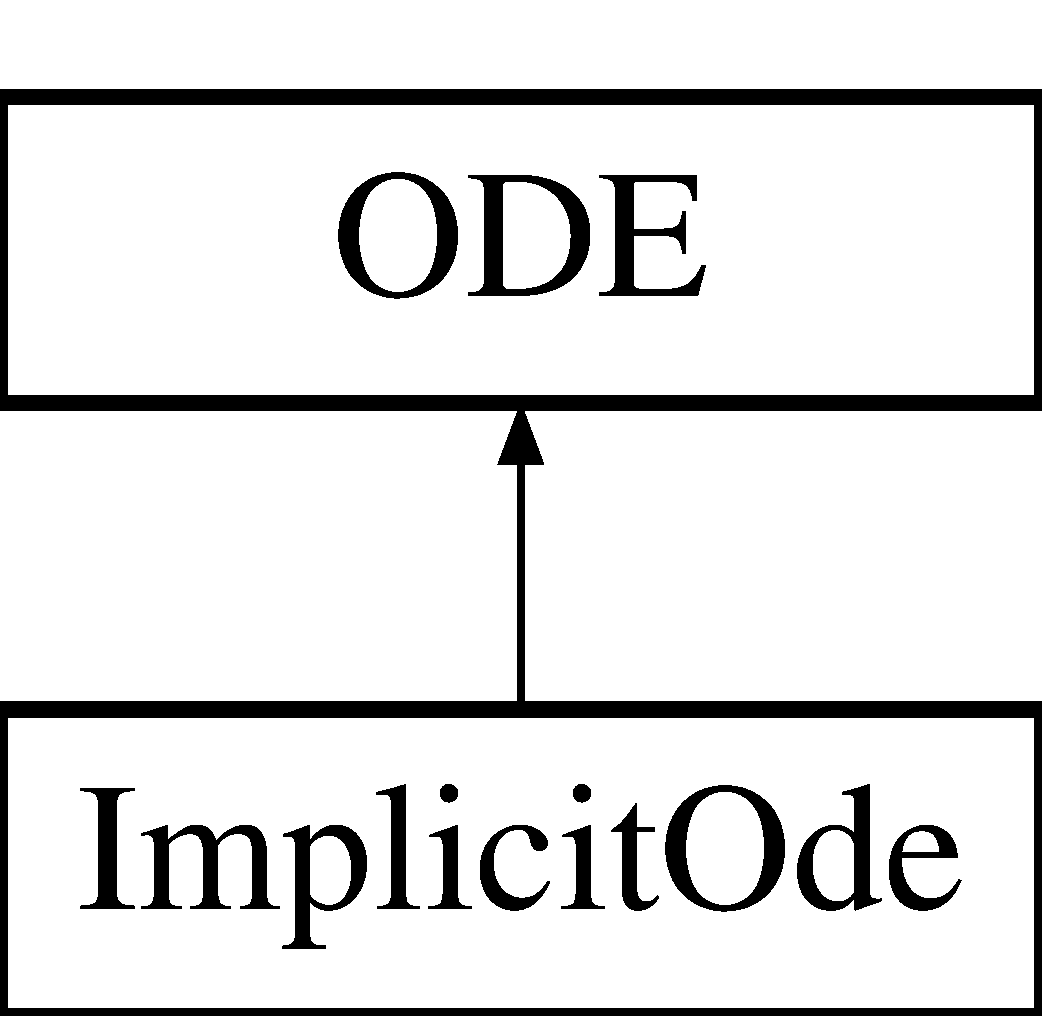
\includegraphics[height=2.000000cm]{classImplicitOde}
\end{center}
\end{figure}
\subsubsection*{Public Member Functions}
\begin{DoxyCompactItemize}
\item 
{\bf Implicit\+Ode} (int my\+\_\+neq, int my\+\_\+nt, double my\+\_\+ti, double my\+\_\+tf, double my\+\_\+dt)
\item 
void {\bf rhs} (double t, double $\ast$u, double $\ast$f)
\item 
void {\bf step} (double t, double $\ast$u, double $\ast$unew)
\end{DoxyCompactItemize}
\subsubsection*{Data Fields}
\begin{DoxyCompactItemize}
\item 
int {\bf neq}
\item 
int {\bf nt}
\item 
double {\bf ti}
\item 
double {\bf tf}
\item 
double {\bf dt}
\end{DoxyCompactItemize}


\subsubsection{Detailed Description}


Definition at line 10 of file implicit.\+cpp.



\subsubsection{Constructor \& Destructor Documentation}
\index{Implicit\+Ode@{Implicit\+Ode}!Implicit\+Ode@{Implicit\+Ode}}
\index{Implicit\+Ode@{Implicit\+Ode}!Implicit\+Ode@{Implicit\+Ode}}
\paragraph[{Implicit\+Ode(int my\+\_\+neq, int my\+\_\+nt, double my\+\_\+ti, double my\+\_\+tf, double my\+\_\+dt)}]{\setlength{\rightskip}{0pt plus 5cm}Implicit\+Ode\+::\+Implicit\+Ode (
\begin{DoxyParamCaption}
\item[{int}]{my\+\_\+neq, }
\item[{int}]{my\+\_\+nt, }
\item[{double}]{my\+\_\+ti, }
\item[{double}]{my\+\_\+tf, }
\item[{double}]{my\+\_\+dt}
\end{DoxyParamCaption}
)\hspace{0.3cm}{\ttfamily [inline]}}\label{classImplicitOde_a39bc33f4917328083edcf86d1f61c7d5}


Definition at line 12 of file implicit.\+cpp.



\subsubsection{Member Function Documentation}
\index{Implicit\+Ode@{Implicit\+Ode}!rhs@{rhs}}
\index{rhs@{rhs}!Implicit\+Ode@{Implicit\+Ode}}
\paragraph[{rhs(double t, double $\ast$u, double $\ast$f)}]{\setlength{\rightskip}{0pt plus 5cm}void Implicit\+Ode\+::rhs (
\begin{DoxyParamCaption}
\item[{double}]{t, }
\item[{double $\ast$}]{u, }
\item[{double $\ast$}]{f}
\end{DoxyParamCaption}
)\hspace{0.3cm}{\ttfamily [inline]}, {\ttfamily [virtual]}}\label{classImplicitOde_a19395eeb6ddb02ef64621b5019bbaf53}
user implemented rhs function, u\textquotesingle{}=rhs(t,u) \begin{DoxyReturn}{Returns}
(by reference) f\+: rhs(t,u) 
\end{DoxyReturn}

\begin{DoxyParams}{Parameters}
{\em t} & current time step \\
\hline
{\em u} & solution u at time t \\
\hline
{\em f} & rhs(t,u) \\
\hline
\end{DoxyParams}


Implements {\bf O\+D\+E} \doxyref{}{p.}{classODE_a9499def749f2914a41b4616f879c991b}.



Definition at line 20 of file implicit.\+cpp.

\index{Implicit\+Ode@{Implicit\+Ode}!step@{step}}
\index{step@{step}!Implicit\+Ode@{Implicit\+Ode}}
\paragraph[{step(double t, double $\ast$u, double $\ast$unew)}]{\setlength{\rightskip}{0pt plus 5cm}void Implicit\+Ode\+::step (
\begin{DoxyParamCaption}
\item[{double}]{t, }
\item[{double $\ast$}]{u, }
\item[{double $\ast$}]{unew}
\end{DoxyParamCaption}
)\hspace{0.3cm}{\ttfamily [inline]}, {\ttfamily [virtual]}}\label{classImplicitOde_a903918de36451c9bf72b0bce1561d5b2}
user implemented step function, for advancing the solution from t to t+dt \begin{DoxyReturn}{Returns}
(by reference) unew\+: solution at time t+dt 
\end{DoxyReturn}

\begin{DoxyParams}{Parameters}
{\em t} & current time step \\
\hline
{\em u} & solution u at time t \\
\hline
{\em unew} & solution at time t+dt \\
\hline
\end{DoxyParams}


Implements {\bf O\+D\+E} \doxyref{}{p.}{classODE_a966f35008ac30511d950b557f53b7468}.



Definition at line 26 of file implicit.\+cpp.



References rhs().



\subsubsection{Field Documentation}
\index{Implicit\+Ode@{Implicit\+Ode}!dt@{dt}}
\index{dt@{dt}!Implicit\+Ode@{Implicit\+Ode}}
\paragraph[{dt}]{\setlength{\rightskip}{0pt plus 5cm}double O\+D\+E\+::dt\hspace{0.3cm}{\ttfamily [inherited]}}\label{classODE_a489591849cd00a583407cde072b51acd}
time step 

Definition at line 33 of file ridc.\+h.



Referenced by Brusselator\+\_\+\+G\+S\+L\+::\+Brusselator\+\_\+\+G\+S\+L(), corr\+\_\+be(), corr\+\_\+fe(), Brusselator\+\_\+\+G\+S\+L\+::jac(), Brusselator\+\_\+\+G\+S\+L\+::newt(), ridc\+\_\+be(), ridc\+\_\+fe(), and Brusselator\+\_\+\+G\+S\+L\+::step().

\index{Implicit\+Ode@{Implicit\+Ode}!neq@{neq}}
\index{neq@{neq}!Implicit\+Ode@{Implicit\+Ode}}
\paragraph[{neq}]{\setlength{\rightskip}{0pt plus 5cm}int O\+D\+E\+::neq\hspace{0.3cm}{\ttfamily [inherited]}}\label{classODE_ad10440423b2185d322223da17d1135c5}
number of equations 

Definition at line 21 of file ridc.\+h.



Referenced by Brusselator\+\_\+\+G\+S\+L\+::\+Brusselator\+\_\+\+G\+S\+L(), corr\+\_\+be(), corr\+\_\+fe(), Brusselator\+\_\+\+G\+S\+L\+::jac(), Brusselator\+\_\+\+G\+S\+L\+::newt(), Brusselator\+\_\+\+G\+S\+L\+::rhs(), ridc\+\_\+be(), ridc\+\_\+fe(), and Brusselator\+\_\+\+G\+S\+L\+::step().

\index{Implicit\+Ode@{Implicit\+Ode}!nt@{nt}}
\index{nt@{nt}!Implicit\+Ode@{Implicit\+Ode}}
\paragraph[{nt}]{\setlength{\rightskip}{0pt plus 5cm}int O\+D\+E\+::nt\hspace{0.3cm}{\ttfamily [inherited]}}\label{classODE_a275faaf08a8602b6a0c60131d3b874b0}
number of time steps 

Definition at line 24 of file ridc.\+h.



Referenced by Brusselator\+\_\+\+G\+S\+L\+::\+Brusselator\+\_\+\+G\+S\+L(), ridc\+\_\+be(), and ridc\+\_\+fe().

\index{Implicit\+Ode@{Implicit\+Ode}!tf@{tf}}
\index{tf@{tf}!Implicit\+Ode@{Implicit\+Ode}}
\paragraph[{tf}]{\setlength{\rightskip}{0pt plus 5cm}double O\+D\+E\+::tf\hspace{0.3cm}{\ttfamily [inherited]}}\label{classODE_aa53beae63fb47d22abca58dd4a407e9e}
final time 

Definition at line 30 of file ridc.\+h.



Referenced by Brusselator\+\_\+\+G\+S\+L\+::\+Brusselator\+\_\+\+G\+S\+L().

\index{Implicit\+Ode@{Implicit\+Ode}!ti@{ti}}
\index{ti@{ti}!Implicit\+Ode@{Implicit\+Ode}}
\paragraph[{ti}]{\setlength{\rightskip}{0pt plus 5cm}double O\+D\+E\+::ti\hspace{0.3cm}{\ttfamily [inherited]}}\label{classODE_abaa6d4b370ec903c7a1f53de5d758cf1}
initial time 

Definition at line 27 of file ridc.\+h.



Referenced by Brusselator\+\_\+\+G\+S\+L\+::\+Brusselator\+\_\+\+G\+S\+L(), ridc\+\_\+be(), and ridc\+\_\+fe().



The documentation for this class was generated from the following file\+:\begin{DoxyCompactItemize}
\item 
examples/implicit/{\bf implicit.\+cpp}\end{DoxyCompactItemize}

\subsection{O\+D\+E Class Reference}
\label{classODE}\index{O\+D\+E@{O\+D\+E}}


{\ttfamily \#include $<$ridc.\+h$>$}

Inheritance diagram for O\+D\+E\+:\begin{figure}[H]
\begin{center}
\leavevmode
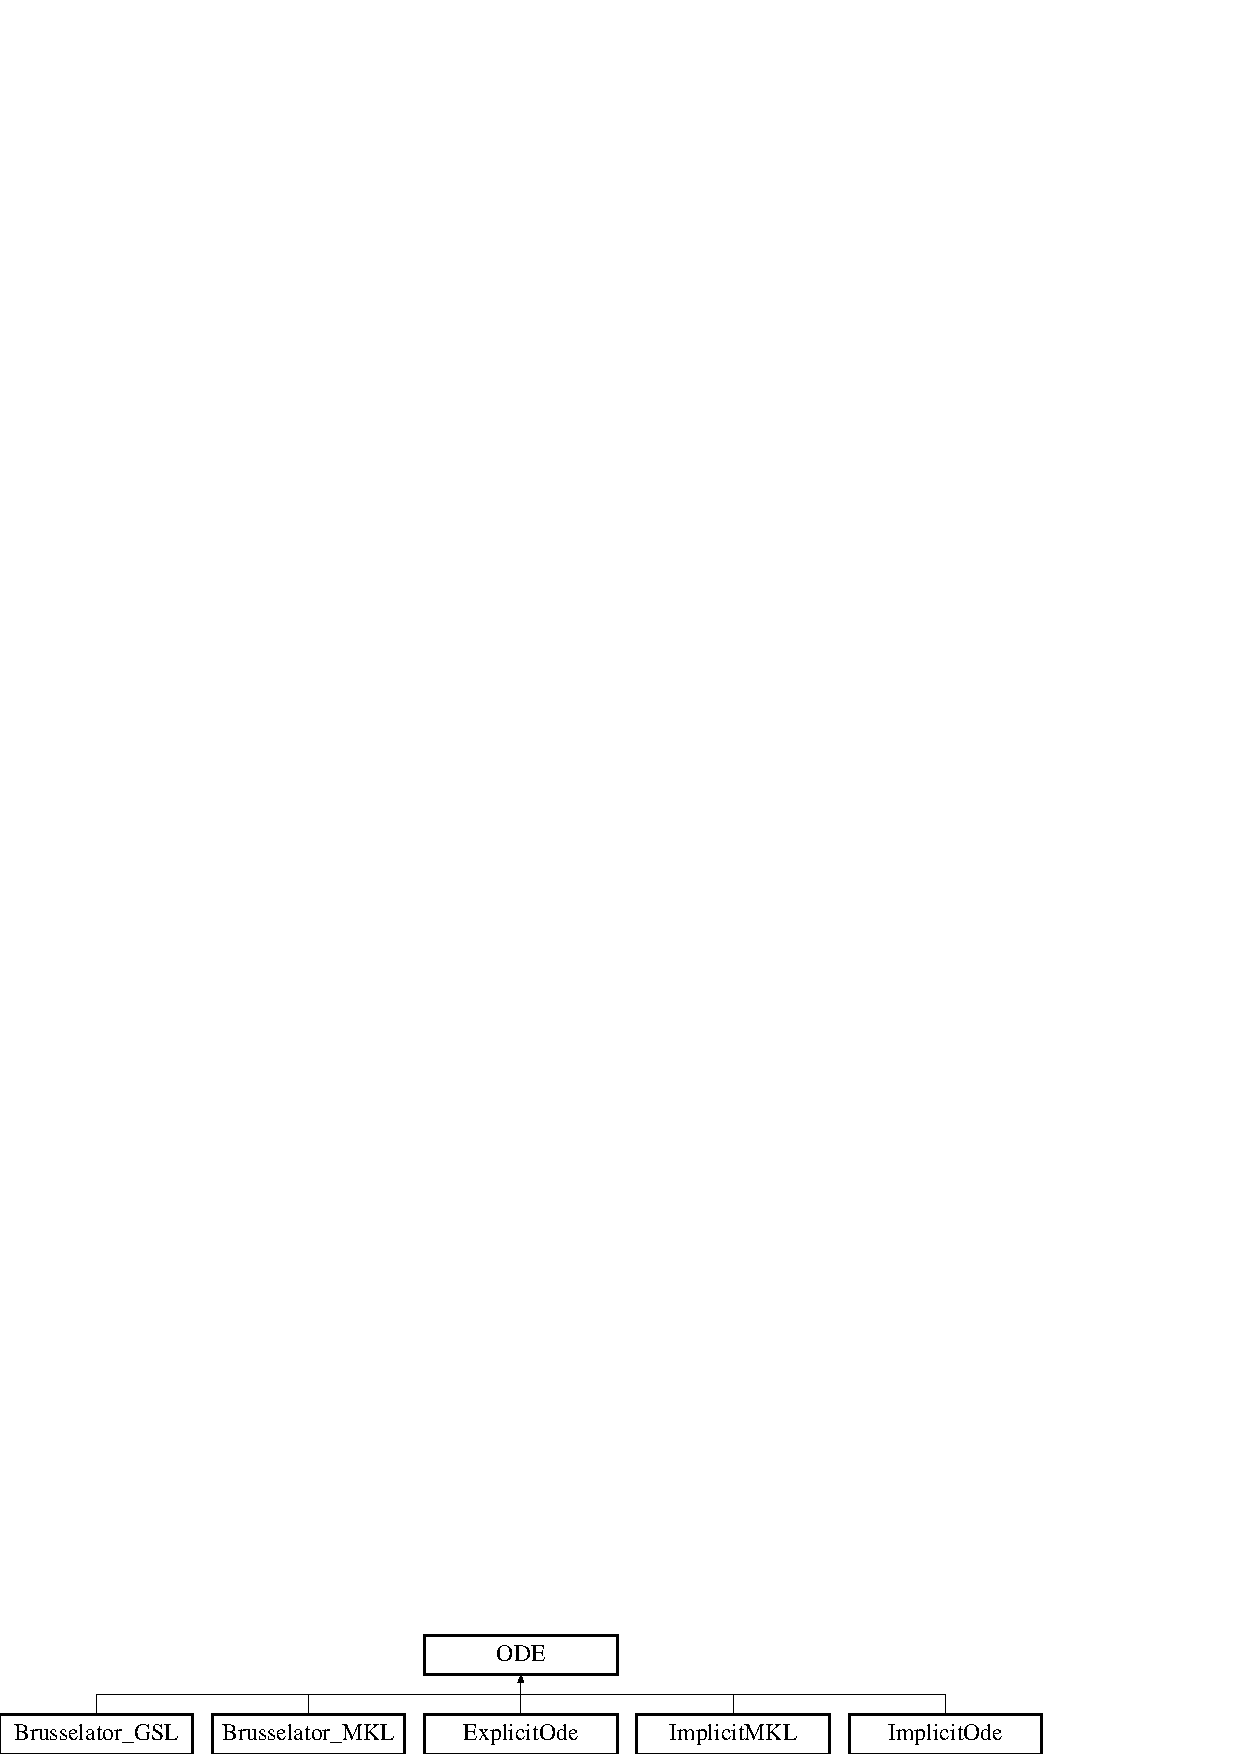
\includegraphics[height=1.914530cm]{classODE}
\end{center}
\end{figure}
\subsubsection*{Public Member Functions}
\begin{DoxyCompactItemize}
\item 
virtual void {\bf rhs} (double t, double $\ast$u, double $\ast$f)=0
\item 
virtual void {\bf step} (double t, double $\ast$u, double $\ast$unew)=0
\end{DoxyCompactItemize}
\subsubsection*{Data Fields}
\begin{DoxyCompactItemize}
\item 
int {\bf neq}
\item 
int {\bf nt}
\item 
double {\bf ti}
\item 
double {\bf tf}
\item 
double {\bf dt}
\end{DoxyCompactItemize}


\subsubsection{Detailed Description}


Definition at line 17 of file ridc.\+h.



\subsubsection{Member Function Documentation}
\index{O\+D\+E@{O\+D\+E}!rhs@{rhs}}
\index{rhs@{rhs}!O\+D\+E@{O\+D\+E}}
\paragraph[{rhs(double t, double $\ast$u, double $\ast$f)=0}]{\setlength{\rightskip}{0pt plus 5cm}virtual void O\+D\+E\+::rhs (
\begin{DoxyParamCaption}
\item[{double}]{t, }
\item[{double $\ast$}]{u, }
\item[{double $\ast$}]{f}
\end{DoxyParamCaption}
)\hspace{0.3cm}{\ttfamily [pure virtual]}}\label{classODE_a9499def749f2914a41b4616f879c991b}
user implemented rhs function, u\textquotesingle{}=rhs(t,u) \begin{DoxyReturn}{Returns}
(by reference) f\+: rhs(t,u) 
\end{DoxyReturn}

\begin{DoxyParams}{Parameters}
{\em t} & current time step \\
\hline
{\em u} & solution u at time t \\
\hline
{\em f} & rhs(t,u) \\
\hline
\end{DoxyParams}


Implemented in {\bf Brusselator\+\_\+\+M\+K\+L} \doxyref{}{p.}{classBrusselator__MKL_a90e55526052241ef810c61cf7ebf382f}, {\bf Implicit\+M\+K\+L} \doxyref{}{p.}{classImplicitMKL_ad5d1c89afc562a0185346ff8e1fe909f}, {\bf Brusselator\+\_\+\+G\+S\+L} \doxyref{}{p.}{classBrusselator__GSL_abee5887ab8e67d01da6bc4ff646dd572}, {\bf Explicit\+Ode} \doxyref{}{p.}{classExplicitOde_a6298c3cda439d026165d08d1c1858ab4}, and {\bf Implicit\+Ode} \doxyref{}{p.}{classImplicitOde_a19395eeb6ddb02ef64621b5019bbaf53}.



Referenced by ridc\+\_\+be(), and ridc\+\_\+fe().

\index{O\+D\+E@{O\+D\+E}!step@{step}}
\index{step@{step}!O\+D\+E@{O\+D\+E}}
\paragraph[{step(double t, double $\ast$u, double $\ast$unew)=0}]{\setlength{\rightskip}{0pt plus 5cm}virtual void O\+D\+E\+::step (
\begin{DoxyParamCaption}
\item[{double}]{t, }
\item[{double $\ast$}]{u, }
\item[{double $\ast$}]{unew}
\end{DoxyParamCaption}
)\hspace{0.3cm}{\ttfamily [pure virtual]}}\label{classODE_a966f35008ac30511d950b557f53b7468}
user implemented step function, for advancing the solution from t to t+dt \begin{DoxyReturn}{Returns}
(by reference) unew\+: solution at time t+dt 
\end{DoxyReturn}

\begin{DoxyParams}{Parameters}
{\em t} & current time step \\
\hline
{\em u} & solution u at time t \\
\hline
{\em unew} & solution at time t+dt \\
\hline
\end{DoxyParams}


Implemented in {\bf Brusselator\+\_\+\+M\+K\+L} \doxyref{}{p.}{classBrusselator__MKL_a3193b7fb7ec213ebd468eafa1e66c020}, {\bf Brusselator\+\_\+\+G\+S\+L} \doxyref{}{p.}{classBrusselator__GSL_a8ed20dea95f4b1705030f0aeee2deacb}, {\bf Implicit\+M\+K\+L} \doxyref{}{p.}{classImplicitMKL_a69936580278402c177332149d044d016}, {\bf Explicit\+Ode} \doxyref{}{p.}{classExplicitOde_af0d28f83df1cbef1a92433389341597b}, and {\bf Implicit\+Ode} \doxyref{}{p.}{classImplicitOde_a903918de36451c9bf72b0bce1561d5b2}.



Referenced by corr\+\_\+be(), corr\+\_\+fe(), ridc\+\_\+be(), and ridc\+\_\+fe().



\subsubsection{Field Documentation}
\index{O\+D\+E@{O\+D\+E}!dt@{dt}}
\index{dt@{dt}!O\+D\+E@{O\+D\+E}}
\paragraph[{dt}]{\setlength{\rightskip}{0pt plus 5cm}double O\+D\+E\+::dt}\label{classODE_a489591849cd00a583407cde072b51acd}
time step 

Definition at line 33 of file ridc.\+h.



Referenced by Brusselator\+\_\+\+G\+S\+L\+::\+Brusselator\+\_\+\+G\+S\+L(), corr\+\_\+be(), corr\+\_\+fe(), Brusselator\+\_\+\+G\+S\+L\+::jac(), Brusselator\+\_\+\+G\+S\+L\+::newt(), ridc\+\_\+be(), ridc\+\_\+fe(), and Brusselator\+\_\+\+G\+S\+L\+::step().

\index{O\+D\+E@{O\+D\+E}!neq@{neq}}
\index{neq@{neq}!O\+D\+E@{O\+D\+E}}
\paragraph[{neq}]{\setlength{\rightskip}{0pt plus 5cm}int O\+D\+E\+::neq}\label{classODE_ad10440423b2185d322223da17d1135c5}
number of equations 

Definition at line 21 of file ridc.\+h.



Referenced by Brusselator\+\_\+\+G\+S\+L\+::\+Brusselator\+\_\+\+G\+S\+L(), corr\+\_\+be(), corr\+\_\+fe(), Brusselator\+\_\+\+G\+S\+L\+::jac(), Brusselator\+\_\+\+G\+S\+L\+::newt(), Brusselator\+\_\+\+G\+S\+L\+::rhs(), ridc\+\_\+be(), ridc\+\_\+fe(), and Brusselator\+\_\+\+G\+S\+L\+::step().

\index{O\+D\+E@{O\+D\+E}!nt@{nt}}
\index{nt@{nt}!O\+D\+E@{O\+D\+E}}
\paragraph[{nt}]{\setlength{\rightskip}{0pt plus 5cm}int O\+D\+E\+::nt}\label{classODE_a275faaf08a8602b6a0c60131d3b874b0}
number of time steps 

Definition at line 24 of file ridc.\+h.



Referenced by Brusselator\+\_\+\+G\+S\+L\+::\+Brusselator\+\_\+\+G\+S\+L(), ridc\+\_\+be(), and ridc\+\_\+fe().

\index{O\+D\+E@{O\+D\+E}!tf@{tf}}
\index{tf@{tf}!O\+D\+E@{O\+D\+E}}
\paragraph[{tf}]{\setlength{\rightskip}{0pt plus 5cm}double O\+D\+E\+::tf}\label{classODE_aa53beae63fb47d22abca58dd4a407e9e}
final time 

Definition at line 30 of file ridc.\+h.



Referenced by Brusselator\+\_\+\+G\+S\+L\+::\+Brusselator\+\_\+\+G\+S\+L().

\index{O\+D\+E@{O\+D\+E}!ti@{ti}}
\index{ti@{ti}!O\+D\+E@{O\+D\+E}}
\paragraph[{ti}]{\setlength{\rightskip}{0pt plus 5cm}double O\+D\+E\+::ti}\label{classODE_abaa6d4b370ec903c7a1f53de5d758cf1}
initial time 

Definition at line 27 of file ridc.\+h.



Referenced by Brusselator\+\_\+\+G\+S\+L\+::\+Brusselator\+\_\+\+G\+S\+L(), ridc\+\_\+be(), and ridc\+\_\+fe().



The documentation for this class was generated from the following file\+:\begin{DoxyCompactItemize}
\item 
src/{\bf ridc.\+h}\end{DoxyCompactItemize}

\subsection{P\+A\+R\+A\+M\+E\+T\+E\+R Struct Reference}
\label{structPARAMETER}\index{P\+A\+R\+A\+M\+E\+T\+E\+R@{P\+A\+R\+A\+M\+E\+T\+E\+R}}


{\ttfamily \#include $<$ode.\+h$>$}

\subsubsection*{Data Fields}
\begin{DoxyCompactItemize}
\item 
int {\bf neq}
\item 
int {\bf nt}
\item 
double {\bf ti}
\item 
double {\bf tf}
\item 
double {\bf dt}
\end{DoxyCompactItemize}


\subsubsection{Detailed Description}
2014--6--18 \doxyref{ode.\+h}{p.}{ode_8h} Requires at least dt -\/ delta t neq -\/ number of equations 

Definition at line 13 of file ode.\+h.



\subsubsection{Field Documentation}
\index{P\+A\+R\+A\+M\+E\+T\+E\+R@{P\+A\+R\+A\+M\+E\+T\+E\+R}!dt@{dt}}
\index{dt@{dt}!P\+A\+R\+A\+M\+E\+T\+E\+R@{P\+A\+R\+A\+M\+E\+T\+E\+R}}
\paragraph[{dt}]{\setlength{\rightskip}{0pt plus 5cm}double P\+A\+R\+A\+M\+E\+T\+E\+R\+::dt}\label{structPARAMETER_a6c8d30eb1e07202b09f07c946753e482}


Definition at line 18 of file ode.\+h.



Referenced by main(), newt(), and step().

\index{P\+A\+R\+A\+M\+E\+T\+E\+R@{P\+A\+R\+A\+M\+E\+T\+E\+R}!neq@{neq}}
\index{neq@{neq}!P\+A\+R\+A\+M\+E\+T\+E\+R@{P\+A\+R\+A\+M\+E\+T\+E\+R}}
\paragraph[{neq}]{\setlength{\rightskip}{0pt plus 5cm}int P\+A\+R\+A\+M\+E\+T\+E\+R\+::neq}\label{structPARAMETER_a8ee37a1980633da35df1c8abfb1ec749}


Definition at line 14 of file ode.\+h.



Referenced by jac(), main(), newt(), rhs(), and step().

\index{P\+A\+R\+A\+M\+E\+T\+E\+R@{P\+A\+R\+A\+M\+E\+T\+E\+R}!nt@{nt}}
\index{nt@{nt}!P\+A\+R\+A\+M\+E\+T\+E\+R@{P\+A\+R\+A\+M\+E\+T\+E\+R}}
\paragraph[{nt}]{\setlength{\rightskip}{0pt plus 5cm}int P\+A\+R\+A\+M\+E\+T\+E\+R\+::nt}\label{structPARAMETER_a2d5f4361422666a88a03950206b5a3ff}


Definition at line 15 of file ode.\+h.



Referenced by main().

\index{P\+A\+R\+A\+M\+E\+T\+E\+R@{P\+A\+R\+A\+M\+E\+T\+E\+R}!tf@{tf}}
\index{tf@{tf}!P\+A\+R\+A\+M\+E\+T\+E\+R@{P\+A\+R\+A\+M\+E\+T\+E\+R}}
\paragraph[{tf}]{\setlength{\rightskip}{0pt plus 5cm}double P\+A\+R\+A\+M\+E\+T\+E\+R\+::tf}\label{structPARAMETER_a59b3b90e4ce6d567e0abd94e52f8aa1b}


Definition at line 17 of file ode.\+h.



Referenced by main().

\index{P\+A\+R\+A\+M\+E\+T\+E\+R@{P\+A\+R\+A\+M\+E\+T\+E\+R}!ti@{ti}}
\index{ti@{ti}!P\+A\+R\+A\+M\+E\+T\+E\+R@{P\+A\+R\+A\+M\+E\+T\+E\+R}}
\paragraph[{ti}]{\setlength{\rightskip}{0pt plus 5cm}double P\+A\+R\+A\+M\+E\+T\+E\+R\+::ti}\label{structPARAMETER_af5efb24886ce50393018b9ccab35f45e}


Definition at line 16 of file ode.\+h.



Referenced by main().



The documentation for this struct was generated from the following file\+:\begin{DoxyCompactItemize}
\item 
examples/brusselator\+\_\+radau\+\_\+mkl/{\bf ode.\+h}\end{DoxyCompactItemize}

\section{File Documentation}
\subsection{doc/source/0\+\_\+installing.md File Reference}
\label{0__installing_8md}\index{doc/source/0\+\_\+installing.\+md@{doc/source/0\+\_\+installing.\+md}}

\subsection{doc/source/1\+\_\+contributing.md File Reference}
\label{1__contributing_8md}\index{doc/source/1\+\_\+contributing.\+md@{doc/source/1\+\_\+contributing.\+md}}

\subsection{doc/source/2\+\_\+running.md File Reference}
\label{2__running_8md}\index{doc/source/2\+\_\+running.\+md@{doc/source/2\+\_\+running.\+md}}

\subsection{doc/source/3\+\_\+use.md File Reference}
\label{3__use_8md}\index{doc/source/3\+\_\+use.\+md@{doc/source/3\+\_\+use.\+md}}

\subsection{examples/brusselator\+\_\+gsl/brusselator.cpp File Reference}
\label{brusselator__gsl_2brusselator_8cpp}\index{examples/brusselator\+\_\+gsl/brusselator.\+cpp@{examples/brusselator\+\_\+gsl/brusselator.\+cpp}}
{\ttfamily \#include $<$stdlib.\+h$>$}\\*
{\ttfamily \#include $<$omp.\+h$>$}\\*
{\ttfamily \#include $<$time.\+h$>$}\\*
{\ttfamily \#include $<$stdio.\+h$>$}\\*
{\ttfamily \#include $<$cmath$>$}\\*
{\ttfamily \#include \char`\"{}ridc.\+h\char`\"{}}\\*
{\ttfamily \#include \char`\"{}brusselator.\+h\char`\"{}}\\*
\subsubsection*{Functions}
\begin{DoxyCompactItemize}
\item 
int {\bf main} (int argc, char $\ast$argv[$\,$])
\end{DoxyCompactItemize}


\subsubsection{Function Documentation}
\index{brusselator\+\_\+gsl/brusselator.\+cpp@{brusselator\+\_\+gsl/brusselator.\+cpp}!main@{main}}
\index{main@{main}!brusselator\+\_\+gsl/brusselator.\+cpp@{brusselator\+\_\+gsl/brusselator.\+cpp}}
\paragraph[{main(int argc, char $\ast$argv[])}]{\setlength{\rightskip}{0pt plus 5cm}int main (
\begin{DoxyParamCaption}
\item[{int}]{argc, }
\item[{char $\ast$}]{argv[$\,$]}
\end{DoxyParamCaption}
)}\label{brusselator__gsl_2brusselator_8cpp_a0ddf1224851353fc92bfbff6f499fa97}


Definition at line 10 of file brusselator.\+cpp.



References ridc\+\_\+be().


\subsection{examples/brusselator\+\_\+mkl/brusselator.cpp File Reference}
\label{brusselator__mkl_2brusselator_8cpp}\index{examples/brusselator\+\_\+mkl/brusselator.\+cpp@{examples/brusselator\+\_\+mkl/brusselator.\+cpp}}
{\ttfamily \#include $<$stdlib.\+h$>$}\\*
{\ttfamily \#include $<$omp.\+h$>$}\\*
{\ttfamily \#include $<$time.\+h$>$}\\*
{\ttfamily \#include $<$stdio.\+h$>$}\\*
{\ttfamily \#include \char`\"{}mkl.\+h\char`\"{}}\\*
{\ttfamily \#include \char`\"{}mkl\+\_\+lapacke.\+h\char`\"{}}\\*
{\ttfamily \#include $<$cmath$>$}\\*
{\ttfamily \#include \char`\"{}ridc.\+h\char`\"{}}\\*
{\ttfamily \#include \char`\"{}brusselator.\+h\char`\"{}}\\*
\subsubsection*{Functions}
\begin{DoxyCompactItemize}
\item 
int {\bf main} (int argc, char $\ast$argv[$\,$])
\end{DoxyCompactItemize}


\subsubsection{Function Documentation}
\index{brusselator\+\_\+mkl/brusselator.\+cpp@{brusselator\+\_\+mkl/brusselator.\+cpp}!main@{main}}
\index{main@{main}!brusselator\+\_\+mkl/brusselator.\+cpp@{brusselator\+\_\+mkl/brusselator.\+cpp}}
\paragraph[{main(int argc, char $\ast$argv[])}]{\setlength{\rightskip}{0pt plus 5cm}int main (
\begin{DoxyParamCaption}
\item[{int}]{argc, }
\item[{char $\ast$}]{argv[$\,$]}
\end{DoxyParamCaption}
)}\label{brusselator__mkl_2brusselator_8cpp_a0ddf1224851353fc92bfbff6f499fa97}


Definition at line 12 of file brusselator.\+cpp.



References ridc\+\_\+be().


\subsection{examples/brusselator\+\_\+radau\+\_\+mkl/brusselator.cpp File Reference}
\label{brusselator__radau__mkl_2brusselator_8cpp}\index{examples/brusselator\+\_\+radau\+\_\+mkl/brusselator.\+cpp@{examples/brusselator\+\_\+radau\+\_\+mkl/brusselator.\+cpp}}
{\ttfamily \#include $<$stdlib.\+h$>$}\\*
{\ttfamily \#include $<$stdio.\+h$>$}\\*
{\ttfamily \#include \char`\"{}mkl.\+h\char`\"{}}\\*
{\ttfamily \#include \char`\"{}mkl\+\_\+lapacke.\+h\char`\"{}}\\*
{\ttfamily \#include $<$cmath$>$}\\*
{\ttfamily \#include \char`\"{}ode.\+h\char`\"{}}\\*
\subsubsection*{Functions}
\begin{DoxyCompactItemize}
\item 
void {\bf rhs} (double t, double $\ast$u, {\bf P\+A\+R\+A\+M\+E\+T\+E\+R} param, double $\ast$f)
\item 
void {\bf newt} (double t, double $\ast$uprev, double $\ast$Kguess, double $\ast$g, {\bf P\+A\+R\+A\+M\+E\+T\+E\+R} param, {\bf B\+U\+T\+C\+H\+E\+R} rk)
\item 
void {\bf jac} (double t, double $\ast$uprev, double $\ast$Kguess, double $\ast$J, {\bf P\+A\+R\+A\+M\+E\+T\+E\+R} param, {\bf B\+U\+T\+C\+H\+E\+R} rk)
\item 
void {\bf step} (double t, double $\ast$uold, {\bf P\+A\+R\+A\+M\+E\+T\+E\+R} param, double $\ast$unew, {\bf B\+U\+T\+C\+H\+E\+R} rk)
\end{DoxyCompactItemize}


\subsubsection{Function Documentation}
\index{brusselator\+\_\+radau\+\_\+mkl/brusselator.\+cpp@{brusselator\+\_\+radau\+\_\+mkl/brusselator.\+cpp}!jac@{jac}}
\index{jac@{jac}!brusselator\+\_\+radau\+\_\+mkl/brusselator.\+cpp@{brusselator\+\_\+radau\+\_\+mkl/brusselator.\+cpp}}
\paragraph[{jac(double t, double $\ast$uprev, double $\ast$\+Kguess, double $\ast$\+J, P\+A\+R\+A\+M\+E\+T\+E\+R param, B\+U\+T\+C\+H\+E\+R rk)}]{\setlength{\rightskip}{0pt plus 5cm}void jac (
\begin{DoxyParamCaption}
\item[{double}]{t, }
\item[{double $\ast$}]{uprev, }
\item[{double $\ast$}]{Kguess, }
\item[{double $\ast$}]{J, }
\item[{{\bf P\+A\+R\+A\+M\+E\+T\+E\+R}}]{param, }
\item[{{\bf B\+U\+T\+C\+H\+E\+R}}]{rk}
\end{DoxyParamCaption}
)}\label{brusselator__radau__mkl_2brusselator_8cpp_a2f4e36896b92e6193d45ef27b7020780}
Helper function for computing the Jacobian matrix (using finite differences) for advancing the solution from time t(n) to t(n+1) using an implicit R\+K step on a system of equations \begin{DoxyReturn}{Returns}
(by reference) J the Jacobian for the Newton step 
\end{DoxyReturn}

\begin{DoxyParams}{Parameters}
{\em param} & structure containing number of equations, number of time steps, initial and final time, time step \\
\hline
{\em t} & current time step \\
\hline
{\em uprev} & function value at the previous (known) time step \\
\hline
{\em Kguess} & iterated guess for the stage values \\
\hline
{\em J} & Jacobian, returned by reference \\
\hline
{\em rk} & Butcher Tableau coefficients \\
\hline
\end{DoxyParams}


Definition at line 70 of file brusselator.\+cpp.



References P\+A\+R\+A\+M\+E\+T\+E\+R\+::neq, newt(), and B\+U\+T\+C\+H\+E\+R\+::\+S.



Referenced by Implicit\+M\+K\+L\+::step(), Brusselator\+\_\+\+M\+K\+L\+::step(), and step().

\index{brusselator\+\_\+radau\+\_\+mkl/brusselator.\+cpp@{brusselator\+\_\+radau\+\_\+mkl/brusselator.\+cpp}!newt@{newt}}
\index{newt@{newt}!brusselator\+\_\+radau\+\_\+mkl/brusselator.\+cpp@{brusselator\+\_\+radau\+\_\+mkl/brusselator.\+cpp}}
\paragraph[{newt(double t, double $\ast$uprev, double $\ast$\+Kguess, double $\ast$g, P\+A\+R\+A\+M\+E\+T\+E\+R param, B\+U\+T\+C\+H\+E\+R rk)}]{\setlength{\rightskip}{0pt plus 5cm}void newt (
\begin{DoxyParamCaption}
\item[{double}]{t, }
\item[{double $\ast$}]{uprev, }
\item[{double $\ast$}]{Kguess, }
\item[{double $\ast$}]{g, }
\item[{{\bf P\+A\+R\+A\+M\+E\+T\+E\+R}}]{param, }
\item[{{\bf B\+U\+T\+C\+H\+E\+R}}]{rk}
\end{DoxyParamCaption}
)}\label{brusselator__radau__mkl_2brusselator_8cpp_aa04e20511f2366a5ec0bdff1064203d2}
Helper function for advancing the solution from time t(n) to t(n+1) using an implicit R\+K step on a non linear system using a Newton step. \begin{DoxyReturn}{Returns}
(by reference) g distance from the root, returned by reference 
\end{DoxyReturn}

\begin{DoxyParams}{Parameters}
{\em param} & structure containing number of equations, number of time steps, initial and final time, time step \\
\hline
{\em t} & current time step \\
\hline
{\em uprev} & function value at the previous (known) time step \\
\hline
{\em Kguess} & iterated guess for the stage values \\
\hline
{\em rk} & Butcher Tableau coefficients \\
\hline
{\em g} & distance from the root, returned by reference \\
\hline
\end{DoxyParams}


Definition at line 32 of file brusselator.\+cpp.



References B\+U\+T\+C\+H\+E\+R\+::\+A, B\+U\+T\+C\+H\+E\+R\+::c, P\+A\+R\+A\+M\+E\+T\+E\+R\+::dt, P\+A\+R\+A\+M\+E\+T\+E\+R\+::neq, rhs(), and B\+U\+T\+C\+H\+E\+R\+::\+S.



Referenced by jac(), Implicit\+M\+K\+L\+::step(), Brusselator\+\_\+\+M\+K\+L\+::step(), and step().

\index{brusselator\+\_\+radau\+\_\+mkl/brusselator.\+cpp@{brusselator\+\_\+radau\+\_\+mkl/brusselator.\+cpp}!rhs@{rhs}}
\index{rhs@{rhs}!brusselator\+\_\+radau\+\_\+mkl/brusselator.\+cpp@{brusselator\+\_\+radau\+\_\+mkl/brusselator.\+cpp}}
\paragraph[{rhs(double t, double $\ast$u, P\+A\+R\+A\+M\+E\+T\+E\+R param, double $\ast$f)}]{\setlength{\rightskip}{0pt plus 5cm}void rhs (
\begin{DoxyParamCaption}
\item[{double}]{t, }
\item[{double $\ast$}]{u, }
\item[{{\bf P\+A\+R\+A\+M\+E\+T\+E\+R}}]{param, }
\item[{double $\ast$}]{f}
\end{DoxyParamCaption}
)}\label{brusselator__radau__mkl_2brusselator_8cpp_a85cca37916ac01b8648f8a864bafdae5}
rhs function, u\textquotesingle{}=rhs(t,u) \begin{DoxyReturn}{Returns}
(by reference) f rhs(t,u) 
\end{DoxyReturn}

\begin{DoxyParams}{Parameters}
{\em t} & current time step \\
\hline
{\em u} & solution u at time t \\
\hline
{\em f} & rhs(t,u) \\
\hline
{\em param} & structure containing number of equations, number of time steps, initial and final time, time step \\
\hline
\end{DoxyParams}


Definition at line 9 of file brusselator.\+cpp.



References P\+A\+R\+A\+M\+E\+T\+E\+R\+::neq.



Referenced by Implicit\+M\+K\+L\+::jac(), Brusselator\+\_\+\+M\+K\+L\+::jac(), newt(), Implicit\+M\+K\+L\+::newt(), Brusselator\+\_\+\+M\+K\+L\+::newt(), Explicit\+Ode\+::step(), Implicit\+Ode\+::step(), and step().

\index{brusselator\+\_\+radau\+\_\+mkl/brusselator.\+cpp@{brusselator\+\_\+radau\+\_\+mkl/brusselator.\+cpp}!step@{step}}
\index{step@{step}!brusselator\+\_\+radau\+\_\+mkl/brusselator.\+cpp@{brusselator\+\_\+radau\+\_\+mkl/brusselator.\+cpp}}
\paragraph[{step(double t, double $\ast$uold, P\+A\+R\+A\+M\+E\+T\+E\+R param, double $\ast$unew, B\+U\+T\+C\+H\+E\+R rk)}]{\setlength{\rightskip}{0pt plus 5cm}void step (
\begin{DoxyParamCaption}
\item[{double}]{t, }
\item[{double $\ast$}]{uold, }
\item[{{\bf P\+A\+R\+A\+M\+E\+T\+E\+R}}]{param, }
\item[{double $\ast$}]{unew, }
\item[{{\bf B\+U\+T\+C\+H\+E\+R}}]{rk}
\end{DoxyParamCaption}
)}\label{brusselator__radau__mkl_2brusselator_8cpp_add04c1b0f2b2529551dd6fa2ec1a2296}


Definition at line 105 of file brusselator.\+cpp.



References B\+U\+T\+C\+H\+E\+R\+::b, B\+U\+T\+C\+H\+E\+R\+::c, P\+A\+R\+A\+M\+E\+T\+E\+R\+::dt, jac(), P\+A\+R\+A\+M\+E\+T\+E\+R\+::neq, newt(), rhs(), and B\+U\+T\+C\+H\+E\+R\+::\+S.



Referenced by main().


\subsection{examples/brusselator\+\_\+gsl/brusselator.h File Reference}
\label{brusselator__gsl_2brusselator_8h}\index{examples/brusselator\+\_\+gsl/brusselator.\+h@{examples/brusselator\+\_\+gsl/brusselator.\+h}}
{\ttfamily \#include \char`\"{}ridc.\+h\char`\"{}}\\*
{\ttfamily \#include $<$stdlib.\+h$>$}\\*
{\ttfamily \#include $<$stdio.\+h$>$}\\*
{\ttfamily \#include $<$cmath$>$}\\*
{\ttfamily \#include $<$gsl/gsl\+\_\+linalg.\+h$>$}\\*
\subsubsection*{Data Structures}
\begin{DoxyCompactItemize}
\item 
class {\bf Brusselator\+\_\+\+G\+S\+L}
\end{DoxyCompactItemize}

\subsection{examples/brusselator\+\_\+mkl/brusselator.h File Reference}
\label{brusselator__mkl_2brusselator_8h}\index{examples/brusselator\+\_\+mkl/brusselator.\+h@{examples/brusselator\+\_\+mkl/brusselator.\+h}}
{\ttfamily \#include \char`\"{}ridc.\+h\char`\"{}}\\*
{\ttfamily \#include $<$stdio.\+h$>$}\\*
{\ttfamily \#include \char`\"{}mkl.\+h\char`\"{}}\\*
{\ttfamily \#include \char`\"{}mkl\+\_\+lapacke.\+h\char`\"{}}\\*
\subsubsection*{Data Structures}
\begin{DoxyCompactItemize}
\item 
class {\bf Brusselator\+\_\+\+M\+K\+L}
\end{DoxyCompactItemize}
\subsubsection*{Macros}
\begin{DoxyCompactItemize}
\item 
\#define {\bf \+\_\+\+B\+R\+U\+S\+S\+E\+L\+A\+T\+O\+R\+\_\+\+H\+\_\+}
\end{DoxyCompactItemize}


\subsubsection{Macro Definition Documentation}
\index{brusselator\+\_\+mkl/brusselator.\+h@{brusselator\+\_\+mkl/brusselator.\+h}!\+\_\+\+B\+R\+U\+S\+S\+E\+L\+A\+T\+O\+R\+\_\+\+H\+\_\+@{\+\_\+\+B\+R\+U\+S\+S\+E\+L\+A\+T\+O\+R\+\_\+\+H\+\_\+}}
\index{\+\_\+\+B\+R\+U\+S\+S\+E\+L\+A\+T\+O\+R\+\_\+\+H\+\_\+@{\+\_\+\+B\+R\+U\+S\+S\+E\+L\+A\+T\+O\+R\+\_\+\+H\+\_\+}!brusselator\+\_\+mkl/brusselator.\+h@{brusselator\+\_\+mkl/brusselator.\+h}}
\paragraph[{\+\_\+\+B\+R\+U\+S\+S\+E\+L\+A\+T\+O\+R\+\_\+\+H\+\_\+}]{\setlength{\rightskip}{0pt plus 5cm}\#define \+\_\+\+B\+R\+U\+S\+S\+E\+L\+A\+T\+O\+R\+\_\+\+H\+\_\+}\label{brusselator__mkl_2brusselator_8h_a812147959eafc576a0f4ebed8ae4d0ca}


Definition at line 7 of file brusselator.\+h.


\subsection{examples/brusselator\+\_\+radau\+\_\+mkl/ode.h File Reference}
\label{ode_8h}\index{examples/brusselator\+\_\+radau\+\_\+mkl/ode.\+h@{examples/brusselator\+\_\+radau\+\_\+mkl/ode.\+h}}
\subsubsection*{Data Structures}
\begin{DoxyCompactItemize}
\item 
struct {\bf P\+A\+R\+A\+M\+E\+T\+E\+R}
\item 
struct {\bf B\+U\+T\+C\+H\+E\+R}
\end{DoxyCompactItemize}
\subsubsection*{Functions}
\begin{DoxyCompactItemize}
\item 
void {\bf rhs} (double t, double $\ast$u, {\bf P\+A\+R\+A\+M\+E\+T\+E\+R} param, double $\ast$f)
\item 
void {\bf newt} (double t, double $\ast$uprev, double $\ast$Kguess, double $\ast$g, {\bf P\+A\+R\+A\+M\+E\+T\+E\+R} param, {\bf B\+U\+T\+C\+H\+E\+R} rk)
\item 
void {\bf jac} (double t, double $\ast$uprev, double $\ast$Kguess, double $\ast$J, {\bf P\+A\+R\+A\+M\+E\+T\+E\+R} param, {\bf B\+U\+T\+C\+H\+E\+R} rk)
\item 
void {\bf step} (double t, double $\ast$u, {\bf P\+A\+R\+A\+M\+E\+T\+E\+R} param, double $\ast$unew, {\bf B\+U\+T\+C\+H\+E\+R} rk)
\end{DoxyCompactItemize}


\subsubsection{Function Documentation}
\index{ode.\+h@{ode.\+h}!jac@{jac}}
\index{jac@{jac}!ode.\+h@{ode.\+h}}
\paragraph[{jac(double t, double $\ast$uprev, double $\ast$\+Kguess, double $\ast$\+J, P\+A\+R\+A\+M\+E\+T\+E\+R param, B\+U\+T\+C\+H\+E\+R rk)}]{\setlength{\rightskip}{0pt plus 5cm}void jac (
\begin{DoxyParamCaption}
\item[{double}]{t, }
\item[{double $\ast$}]{uprev, }
\item[{double $\ast$}]{Kguess, }
\item[{double $\ast$}]{J, }
\item[{{\bf P\+A\+R\+A\+M\+E\+T\+E\+R}}]{param, }
\item[{{\bf B\+U\+T\+C\+H\+E\+R}}]{rk}
\end{DoxyParamCaption}
)}\label{ode_8h_a2f4e36896b92e6193d45ef27b7020780}
Helper function for computing the Jacobian matrix (using finite differences) for advancing the solution from time t(n) to t(n+1) using an implicit R\+K step on a system of equations \begin{DoxyReturn}{Returns}
(by reference) J the Jacobian for the Newton step 
\end{DoxyReturn}

\begin{DoxyParams}{Parameters}
{\em param} & structure containing number of equations, number of time steps, initial and final time, time step \\
\hline
{\em t} & current time step \\
\hline
{\em uprev} & function value at the previous (known) time step \\
\hline
{\em Kguess} & iterated guess for the stage values \\
\hline
{\em J} & Jacobian, returned by reference \\
\hline
{\em rk} & Butcher Tableau coefficients \\
\hline
\end{DoxyParams}


Definition at line 70 of file brusselator.\+cpp.



References P\+A\+R\+A\+M\+E\+T\+E\+R\+::neq, newt(), and B\+U\+T\+C\+H\+E\+R\+::\+S.



Referenced by Implicit\+M\+K\+L\+::step(), Brusselator\+\_\+\+M\+K\+L\+::step(), and step().

\index{ode.\+h@{ode.\+h}!newt@{newt}}
\index{newt@{newt}!ode.\+h@{ode.\+h}}
\paragraph[{newt(double t, double $\ast$uprev, double $\ast$\+Kguess, double $\ast$g, P\+A\+R\+A\+M\+E\+T\+E\+R param, B\+U\+T\+C\+H\+E\+R rk)}]{\setlength{\rightskip}{0pt plus 5cm}void newt (
\begin{DoxyParamCaption}
\item[{double}]{t, }
\item[{double $\ast$}]{uprev, }
\item[{double $\ast$}]{Kguess, }
\item[{double $\ast$}]{g, }
\item[{{\bf P\+A\+R\+A\+M\+E\+T\+E\+R}}]{param, }
\item[{{\bf B\+U\+T\+C\+H\+E\+R}}]{rk}
\end{DoxyParamCaption}
)}\label{ode_8h_aa04e20511f2366a5ec0bdff1064203d2}
Helper function for advancing the solution from time t(n) to t(n+1) using an implicit R\+K step on a non linear system using a Newton step. \begin{DoxyReturn}{Returns}
(by reference) g distance from the root, returned by reference 
\end{DoxyReturn}

\begin{DoxyParams}{Parameters}
{\em param} & structure containing number of equations, number of time steps, initial and final time, time step \\
\hline
{\em t} & current time step \\
\hline
{\em uprev} & function value at the previous (known) time step \\
\hline
{\em Kguess} & iterated guess for the stage values \\
\hline
{\em rk} & Butcher Tableau coefficients \\
\hline
{\em g} & distance from the root, returned by reference \\
\hline
\end{DoxyParams}


Definition at line 32 of file brusselator.\+cpp.



References B\+U\+T\+C\+H\+E\+R\+::\+A, B\+U\+T\+C\+H\+E\+R\+::c, P\+A\+R\+A\+M\+E\+T\+E\+R\+::dt, P\+A\+R\+A\+M\+E\+T\+E\+R\+::neq, rhs(), and B\+U\+T\+C\+H\+E\+R\+::\+S.



Referenced by jac(), Implicit\+M\+K\+L\+::step(), Brusselator\+\_\+\+M\+K\+L\+::step(), and step().

\index{ode.\+h@{ode.\+h}!rhs@{rhs}}
\index{rhs@{rhs}!ode.\+h@{ode.\+h}}
\paragraph[{rhs(double t, double $\ast$u, P\+A\+R\+A\+M\+E\+T\+E\+R param, double $\ast$f)}]{\setlength{\rightskip}{0pt plus 5cm}void rhs (
\begin{DoxyParamCaption}
\item[{double}]{t, }
\item[{double $\ast$}]{u, }
\item[{{\bf P\+A\+R\+A\+M\+E\+T\+E\+R}}]{param, }
\item[{double $\ast$}]{f}
\end{DoxyParamCaption}
)}\label{ode_8h_a85cca37916ac01b8648f8a864bafdae5}
rhs function, u\textquotesingle{}=rhs(t,u) \begin{DoxyReturn}{Returns}
(by reference) f rhs(t,u) 
\end{DoxyReturn}

\begin{DoxyParams}{Parameters}
{\em t} & current time step \\
\hline
{\em u} & solution u at time t \\
\hline
{\em f} & rhs(t,u) \\
\hline
{\em param} & structure containing number of equations, number of time steps, initial and final time, time step \\
\hline
\end{DoxyParams}


Definition at line 9 of file brusselator.\+cpp.



References P\+A\+R\+A\+M\+E\+T\+E\+R\+::neq.



Referenced by Implicit\+M\+K\+L\+::jac(), Brusselator\+\_\+\+M\+K\+L\+::jac(), newt(), Implicit\+M\+K\+L\+::newt(), Brusselator\+\_\+\+M\+K\+L\+::newt(), Explicit\+Ode\+::step(), Implicit\+Ode\+::step(), and step().

\index{ode.\+h@{ode.\+h}!step@{step}}
\index{step@{step}!ode.\+h@{ode.\+h}}
\paragraph[{step(double t, double $\ast$u, P\+A\+R\+A\+M\+E\+T\+E\+R param, double $\ast$unew, B\+U\+T\+C\+H\+E\+R rk)}]{\setlength{\rightskip}{0pt plus 5cm}void step (
\begin{DoxyParamCaption}
\item[{double}]{t, }
\item[{double $\ast$}]{u, }
\item[{{\bf P\+A\+R\+A\+M\+E\+T\+E\+R}}]{param, }
\item[{double $\ast$}]{unew, }
\item[{{\bf B\+U\+T\+C\+H\+E\+R}}]{rk}
\end{DoxyParamCaption}
)}\label{ode_8h_a02a2cfd5bf4a4c35f861e2c2d2dab18e}


Definition at line 105 of file brusselator.\+cpp.



References B\+U\+T\+C\+H\+E\+R\+::b, B\+U\+T\+C\+H\+E\+R\+::c, P\+A\+R\+A\+M\+E\+T\+E\+R\+::dt, jac(), P\+A\+R\+A\+M\+E\+T\+E\+R\+::neq, newt(), rhs(), and B\+U\+T\+C\+H\+E\+R\+::\+S.



Referenced by main().


\subsection{examples/brusselator\+\_\+radau\+\_\+mkl/radau.cpp File Reference}
\label{radau_8cpp}\index{examples/brusselator\+\_\+radau\+\_\+mkl/radau.\+cpp@{examples/brusselator\+\_\+radau\+\_\+mkl/radau.\+cpp}}
{\ttfamily \#include $<$stdlib.\+h$>$}\\*
{\ttfamily \#include $<$time.\+h$>$}\\*
{\ttfamily \#include $<$stdio.\+h$>$}\\*
{\ttfamily \#include \char`\"{}mkl.\+h\char`\"{}}\\*
{\ttfamily \#include \char`\"{}mkl\+\_\+lapacke.\+h\char`\"{}}\\*
{\ttfamily \#include $<$cmath$>$}\\*
{\ttfamily \#include \char`\"{}ode.\+h\char`\"{}}\\*
\subsubsection*{Functions}
\begin{DoxyCompactItemize}
\item 
int {\bf main} (int argc, char $\ast$argv[$\,$])
\begin{DoxyCompactList}\small\item\em This is the the main function for the brusselator\+\_\+radau\+\_\+mkl example. \end{DoxyCompactList}\end{DoxyCompactItemize}


\subsubsection{Function Documentation}
\index{radau.\+cpp@{radau.\+cpp}!main@{main}}
\index{main@{main}!radau.\+cpp@{radau.\+cpp}}
\paragraph[{main(int argc, char $\ast$argv[])}]{\setlength{\rightskip}{0pt plus 5cm}int main (
\begin{DoxyParamCaption}
\item[{int}]{argc, }
\item[{char $\ast$}]{argv[$\,$]}
\end{DoxyParamCaption}
)}\label{radau_8cpp_a0ddf1224851353fc92bfbff6f499fa97}


This is the the main function for the brusselator\+\_\+radau\+\_\+mkl example. 

This will pass user given options along with some standard options for this type of problem in to the \doxyref{P\+A\+R\+A\+M\+E\+T\+E\+R}{p.}{structPARAMETER} struct and start the solving the problem 

Definition at line 17 of file radau.\+cpp.



References B\+U\+T\+C\+H\+E\+R\+::\+A, B\+U\+T\+C\+H\+E\+R\+::b, B\+U\+T\+C\+H\+E\+R\+::c, P\+A\+R\+A\+M\+E\+T\+E\+R\+::dt, P\+A\+R\+A\+M\+E\+T\+E\+R\+::neq, P\+A\+R\+A\+M\+E\+T\+E\+R\+::nt, B\+U\+T\+C\+H\+E\+R\+::\+S, step(), P\+A\+R\+A\+M\+E\+T\+E\+R\+::tf, and P\+A\+R\+A\+M\+E\+T\+E\+R\+::ti.


\subsection{examples/explicit/explicit.cpp File Reference}
\label{explicit_8cpp}\index{examples/explicit/explicit.\+cpp@{examples/explicit/explicit.\+cpp}}
{\ttfamily \#include $<$stdlib.\+h$>$}\\*
{\ttfamily \#include $<$omp.\+h$>$}\\*
{\ttfamily \#include $<$time.\+h$>$}\\*
{\ttfamily \#include $<$stdio.\+h$>$}\\*
{\ttfamily \#include \char`\"{}ridc.\+h\char`\"{}}\\*
\subsubsection*{Data Structures}
\begin{DoxyCompactItemize}
\item 
class {\bf Explicit\+Ode}
\end{DoxyCompactItemize}
\subsubsection*{Functions}
\begin{DoxyCompactItemize}
\item 
int {\bf main} (int argc, char $\ast$argv[$\,$])
\end{DoxyCompactItemize}


\subsubsection{Function Documentation}
\index{explicit.\+cpp@{explicit.\+cpp}!main@{main}}
\index{main@{main}!explicit.\+cpp@{explicit.\+cpp}}
\paragraph[{main(int argc, char $\ast$argv[])}]{\setlength{\rightskip}{0pt plus 5cm}int main (
\begin{DoxyParamCaption}
\item[{int}]{argc, }
\item[{char $\ast$}]{argv[$\,$]}
\end{DoxyParamCaption}
)}\label{explicit_8cpp_a0ddf1224851353fc92bfbff6f499fa97}


Definition at line 38 of file explicit.\+cpp.



References ridc\+\_\+fe().


\subsection{examples/implicit/implicit.cpp File Reference}
\label{implicit_8cpp}\index{examples/implicit/implicit.\+cpp@{examples/implicit/implicit.\+cpp}}
{\ttfamily \#include $<$stdlib.\+h$>$}\\*
{\ttfamily \#include $<$omp.\+h$>$}\\*
{\ttfamily \#include $<$time.\+h$>$}\\*
{\ttfamily \#include $<$stdio.\+h$>$}\\*
{\ttfamily \#include \char`\"{}ridc.\+h\char`\"{}}\\*
\subsubsection*{Data Structures}
\begin{DoxyCompactItemize}
\item 
class {\bf Implicit\+Ode}
\end{DoxyCompactItemize}
\subsubsection*{Functions}
\begin{DoxyCompactItemize}
\item 
int {\bf main} (int argc, char $\ast$argv[$\,$])
\end{DoxyCompactItemize}


\subsubsection{Function Documentation}
\index{implicit.\+cpp@{implicit.\+cpp}!main@{main}}
\index{main@{main}!implicit.\+cpp@{implicit.\+cpp}}
\paragraph[{main(int argc, char $\ast$argv[])}]{\setlength{\rightskip}{0pt plus 5cm}int main (
\begin{DoxyParamCaption}
\item[{int}]{argc, }
\item[{char $\ast$}]{argv[$\,$]}
\end{DoxyParamCaption}
)}\label{implicit_8cpp_a0ddf1224851353fc92bfbff6f499fa97}


Definition at line 39 of file implicit.\+cpp.



References ridc\+\_\+be().


\subsection{examples/implicit\+\_\+mkl/implicit.cpp File Reference}
\label{mkl_2implicit_8cpp}\index{examples/implicit\+\_\+mkl/implicit.\+cpp@{examples/implicit\+\_\+mkl/implicit.\+cpp}}
{\ttfamily \#include $<$stdlib.\+h$>$}\\*
{\ttfamily \#include $<$omp.\+h$>$}\\*
{\ttfamily \#include $<$time.\+h$>$}\\*
{\ttfamily \#include $<$stdio.\+h$>$}\\*
{\ttfamily \#include \char`\"{}ridc.\+h\char`\"{}}\\*
{\ttfamily \#include \char`\"{}implicit.\+h\char`\"{}}\\*
\subsubsection*{Functions}
\begin{DoxyCompactItemize}
\item 
int {\bf main} (int argc, char $\ast$argv[$\,$])
\end{DoxyCompactItemize}


\subsubsection{Function Documentation}
\index{mkl/implicit.\+cpp@{mkl/implicit.\+cpp}!main@{main}}
\index{main@{main}!mkl/implicit.\+cpp@{mkl/implicit.\+cpp}}
\paragraph[{main(int argc, char $\ast$argv[])}]{\setlength{\rightskip}{0pt plus 5cm}int main (
\begin{DoxyParamCaption}
\item[{int}]{argc, }
\item[{char $\ast$}]{argv[$\,$]}
\end{DoxyParamCaption}
)}\label{mkl_2implicit_8cpp_a0ddf1224851353fc92bfbff6f499fa97}


Definition at line 8 of file implicit.\+cpp.



References ridc\+\_\+be().


\subsection{examples/implicit\+\_\+mkl/implicit.h File Reference}
\label{implicit_8h}\index{examples/implicit\+\_\+mkl/implicit.\+h@{examples/implicit\+\_\+mkl/implicit.\+h}}
{\ttfamily \#include \char`\"{}ridc.\+h\char`\"{}}\\*
{\ttfamily \#include $<$stdio.\+h$>$}\\*
{\ttfamily \#include \char`\"{}mkl.\+h\char`\"{}}\\*
{\ttfamily \#include \char`\"{}mkl\+\_\+lapacke.\+h\char`\"{}}\\*
\subsubsection*{Data Structures}
\begin{DoxyCompactItemize}
\item 
class {\bf Implicit\+M\+K\+L}
\end{DoxyCompactItemize}
\subsubsection*{Macros}
\begin{DoxyCompactItemize}
\item 
\#define {\bf \+\_\+\+I\+M\+P\+L\+I\+C\+I\+T\+\_\+\+H\+\_\+}
\end{DoxyCompactItemize}


\subsubsection{Macro Definition Documentation}
\index{implicit.\+h@{implicit.\+h}!\+\_\+\+I\+M\+P\+L\+I\+C\+I\+T\+\_\+\+H\+\_\+@{\+\_\+\+I\+M\+P\+L\+I\+C\+I\+T\+\_\+\+H\+\_\+}}
\index{\+\_\+\+I\+M\+P\+L\+I\+C\+I\+T\+\_\+\+H\+\_\+@{\+\_\+\+I\+M\+P\+L\+I\+C\+I\+T\+\_\+\+H\+\_\+}!implicit.\+h@{implicit.\+h}}
\paragraph[{\+\_\+\+I\+M\+P\+L\+I\+C\+I\+T\+\_\+\+H\+\_\+}]{\setlength{\rightskip}{0pt plus 5cm}\#define \+\_\+\+I\+M\+P\+L\+I\+C\+I\+T\+\_\+\+H\+\_\+}\label{implicit_8h_ae86b67c4f0c0cc9a5f89ed888e72b8d0}


Definition at line 7 of file implicit.\+h.


\subsection{R\+E\+A\+D\+M\+E.\+md File Reference}
\label{README_8md}\index{R\+E\+A\+D\+M\+E.\+md@{R\+E\+A\+D\+M\+E.\+md}}

\subsection{src/ridc.cpp File Reference}
\label{ridc_8cpp}\index{src/ridc.\+cpp@{src/ridc.\+cpp}}
{\ttfamily \#include \char`\"{}ridc.\+h\char`\"{}}\\*
{\ttfamily \#include $<$stdio.\+h$>$}\\*
\subsubsection*{Functions}
\begin{DoxyCompactItemize}
\item 
void {\bf ridc\+\_\+fe} ({\bf O\+D\+E} $\ast$ode, int order, double $\ast$sol)
\item 
void {\bf ridc\+\_\+be} ({\bf O\+D\+E} $\ast$ode, int order, double $\ast$sol)
\item 
void {\bf lagrange\+\_\+coeff} (double $\ast$x, int Nx, int i, double $\ast$L)
\item 
double {\bf get\+\_\+quad\+\_\+weight} (double $\ast$L, int Nx, double a, double b)
\item 
void {\bf integration\+\_\+matrices} (int N, double $\ast$$\ast$S)
\item 
void {\bf init\+\_\+unif\+\_\+nodes} (double $\ast$x, int Nx, double a, double b)
\item 
void {\bf corr\+\_\+fe} ({\bf O\+D\+E} $\ast$ode, double $\ast$uold, double $\ast$$\ast$fprev, double $\ast$$\ast$S, int index, int level, double t, double $\ast$unew)
\item 
void {\bf corr\+\_\+be} ({\bf O\+D\+E} $\ast$ode, double $\ast$uold, double $\ast$$\ast$fprev, double $\ast$$\ast$S, int index, int level, double t, double $\ast$unew)
\end{DoxyCompactItemize}


\subsubsection{Function Documentation}
\index{ridc.\+cpp@{ridc.\+cpp}!corr\+\_\+be@{corr\+\_\+be}}
\index{corr\+\_\+be@{corr\+\_\+be}!ridc.\+cpp@{ridc.\+cpp}}
\paragraph[{corr\+\_\+be(\+O\+D\+E $\ast$ode, double $\ast$uold, double $\ast$$\ast$fprev, double $\ast$$\ast$\+S, int index, int level, double t, double $\ast$unew)}]{\setlength{\rightskip}{0pt plus 5cm}void corr\+\_\+be (
\begin{DoxyParamCaption}
\item[{{\bf O\+D\+E} $\ast$}]{ode, }
\item[{double $\ast$}]{uold, }
\item[{double $\ast$$\ast$}]{fprev, }
\item[{double $\ast$$\ast$}]{S, }
\item[{int}]{index, }
\item[{int}]{level, }
\item[{double}]{t, }
\item[{double $\ast$}]{unew}
\end{DoxyParamCaption}
)}\label{ridc_8cpp_a8f0874733447d234c1f21129a19c5630}
R\+I\+D\+C helper function -\/ solves error equation, updating the solution from time t to time t+param.dt.

\begin{DoxyReturn}{Returns}
(by reference) unew\+: solution at time level t + param.\+dt
\end{DoxyReturn}

\begin{DoxyParams}{Parameters}
{\em ode} & abstract class containing parameters and step/rhs functions \\
\hline
{\em uold} & solution at time level t \\
\hline
{\em fprev} & matrix containing derivative information from previous steps, previous level \\
\hline
{\em S} & integration matrix (quadrature weights) \\
\hline
{\em index} & decides which quadrature weights to use \\
\hline
{\em level} & determines size of quadrature stencil \\
\hline
{\em t} & current time iterate \\
\hline
{\em unew} & solution at the new time level, passed by reference \\
\hline
\end{DoxyParams}


Definition at line 894 of file ridc.\+cpp.



References O\+D\+E\+::dt, O\+D\+E\+::neq, and O\+D\+E\+::step().



Referenced by ridc\+\_\+be().

\index{ridc.\+cpp@{ridc.\+cpp}!corr\+\_\+fe@{corr\+\_\+fe}}
\index{corr\+\_\+fe@{corr\+\_\+fe}!ridc.\+cpp@{ridc.\+cpp}}
\paragraph[{corr\+\_\+fe(\+O\+D\+E $\ast$ode, double $\ast$uold, double $\ast$$\ast$fprev, double $\ast$$\ast$\+S, int index, int level, double t, double $\ast$unew)}]{\setlength{\rightskip}{0pt plus 5cm}void corr\+\_\+fe (
\begin{DoxyParamCaption}
\item[{{\bf O\+D\+E} $\ast$}]{ode, }
\item[{double $\ast$}]{uold, }
\item[{double $\ast$$\ast$}]{fprev, }
\item[{double $\ast$$\ast$}]{S, }
\item[{int}]{index, }
\item[{int}]{level, }
\item[{double}]{t, }
\item[{double $\ast$}]{unew}
\end{DoxyParamCaption}
)}\label{ridc_8cpp_a9d505d3e3fe2d373768b906cc207b199}
R\+I\+D\+C helper function -\/ solves error equation, updating the solution from time t to time t+param.dt.

\begin{DoxyReturn}{Returns}
(by reference) unew\+: solution at time level t + param.\+dt
\end{DoxyReturn}

\begin{DoxyParams}{Parameters}
{\em ode} & abstract class containing parameters and step/rhs functions \\
\hline
{\em uold} & solution at time level t \\
\hline
{\em fprev} & matrix containing derivative information from previous steps, previous level \\
\hline
{\em S} & integration matrix (quadrature weights) \\
\hline
{\em index} & decides which quadrature weights to use \\
\hline
{\em level} & determines size of quadrature stencil \\
\hline
{\em t} & current time iterate \\
\hline
{\em unew} & solution at the new time level, passed by reference \\
\hline
\end{DoxyParams}


Definition at line 846 of file ridc.\+cpp.



References O\+D\+E\+::dt, O\+D\+E\+::neq, and O\+D\+E\+::step().



Referenced by ridc\+\_\+fe().

\index{ridc.\+cpp@{ridc.\+cpp}!get\+\_\+quad\+\_\+weight@{get\+\_\+quad\+\_\+weight}}
\index{get\+\_\+quad\+\_\+weight@{get\+\_\+quad\+\_\+weight}!ridc.\+cpp@{ridc.\+cpp}}
\paragraph[{get\+\_\+quad\+\_\+weight(double $\ast$\+L, int Nx, double a, double b)}]{\setlength{\rightskip}{0pt plus 5cm}double get\+\_\+quad\+\_\+weight (
\begin{DoxyParamCaption}
\item[{double $\ast$}]{L, }
\item[{int}]{Nx, }
\item[{double}]{a, }
\item[{double}]{b}
\end{DoxyParamCaption}
)}\label{ridc_8cpp_a07e5dce091c0ec540e8f9aff1bbc2a66}
R\+I\+D\+C helper function -- generates quadrature weight, int(L\+\_\+\{n,i\}(x),x=a..b)

\begin{DoxyReturn}{Returns}
quadrature weights
\end{DoxyReturn}

\begin{DoxyParams}{Parameters}
{\em a} & range of integration \\
\hline
{\em b} & range of integration \\
\hline
{\em Nx} & number of quadrature nodes \\
\hline
{\em L} & coefficients for Lagrange poly, L[0] + L[1]x + L[2]x$^\wedge$2 + ... \\
\hline
\end{DoxyParams}


Definition at line 723 of file ridc.\+cpp.



Referenced by integration\+\_\+matrices().

\index{ridc.\+cpp@{ridc.\+cpp}!init\+\_\+unif\+\_\+nodes@{init\+\_\+unif\+\_\+nodes}}
\index{init\+\_\+unif\+\_\+nodes@{init\+\_\+unif\+\_\+nodes}!ridc.\+cpp@{ridc.\+cpp}}
\paragraph[{init\+\_\+unif\+\_\+nodes(double $\ast$x, int Nx, double a, double b)}]{\setlength{\rightskip}{0pt plus 5cm}void init\+\_\+unif\+\_\+nodes (
\begin{DoxyParamCaption}
\item[{double $\ast$}]{x, }
\item[{int}]{Nx, }
\item[{double}]{a, }
\item[{double}]{b}
\end{DoxyParamCaption}
)}\label{ridc_8cpp_a6784be1bca782a9aef5584921af9304c}
R\+I\+D\+C helper function -- initializes uniformly spaced quadrature nodes

\begin{DoxyReturn}{Returns}
(by reference) x\+: uniformly spaced quadrature nodes
\end{DoxyReturn}

\begin{DoxyParams}{Parameters}
{\em Nx} & number of quadrature nodes \\
\hline
{\em a} & range of integration \\
\hline
{\em b} & range of integration \\
\hline
{\em x} & quadrature node location (returned by reference) \\
\hline
\end{DoxyParams}


Definition at line 811 of file ridc.\+cpp.



Referenced by integration\+\_\+matrices().

\index{ridc.\+cpp@{ridc.\+cpp}!integration\+\_\+matrices@{integration\+\_\+matrices}}
\index{integration\+\_\+matrices@{integration\+\_\+matrices}!ridc.\+cpp@{ridc.\+cpp}}
\paragraph[{integration\+\_\+matrices(int N, double $\ast$$\ast$\+S)}]{\setlength{\rightskip}{0pt plus 5cm}void integration\+\_\+matrices (
\begin{DoxyParamCaption}
\item[{int}]{Nx, }
\item[{double $\ast$$\ast$}]{S}
\end{DoxyParamCaption}
)}\label{ridc_8cpp_a4bd004e1c1236beb766757b596fae927}
R\+I\+D\+C helper function -- constructions the integration matrix using get\+\_\+quad\+\_\+weight

\begin{DoxyReturn}{Returns}
(by reference) the integration matrix S
\end{DoxyReturn}

\begin{DoxyParams}{Parameters}
{\em Nx} & number of quadrature nodes \\
\hline
{\em S} & integration matrix (by reference) \\
\hline
\end{DoxyParams}


Definition at line 765 of file ridc.\+cpp.



References get\+\_\+quad\+\_\+weight(), init\+\_\+unif\+\_\+nodes(), and lagrange\+\_\+coeff().



Referenced by ridc\+\_\+be(), and ridc\+\_\+fe().

\index{ridc.\+cpp@{ridc.\+cpp}!lagrange\+\_\+coeff@{lagrange\+\_\+coeff}}
\index{lagrange\+\_\+coeff@{lagrange\+\_\+coeff}!ridc.\+cpp@{ridc.\+cpp}}
\paragraph[{lagrange\+\_\+coeff(double $\ast$x, int Nx, int i, double $\ast$\+L)}]{\setlength{\rightskip}{0pt plus 5cm}void lagrange\+\_\+coeff (
\begin{DoxyParamCaption}
\item[{double $\ast$}]{x, }
\item[{int}]{Nx, }
\item[{int}]{i, }
\item[{double $\ast$}]{L}
\end{DoxyParamCaption}
)}\label{ridc_8cpp_a73647697e05b092fe6d4a43361977b0a}
R\+I\+D\+C helper function -- generates the coefficients for the lagrange interpolatory polynomials.

\begin{DoxyReturn}{Returns}
(by reference) L\+: coefficients for the Lagrange intepolatory polynomial. L is a vector of elements such that p(x) = L(0) + L(1)$\ast$x + L(2)$\ast$x$^\wedge$2 + ... 
\end{DoxyReturn}

\begin{DoxyParams}{Parameters}
{\em x} & quadrature nodes \\
\hline
{\em i} & the i$^\wedge$\{th\} Lagrange polynomial \\
\hline
{\em Nx} & number of quadrature nodes \\
\hline
{\em L} & coefficients, returned by reference \\
\hline
\end{DoxyParams}


Definition at line 652 of file ridc.\+cpp.



Referenced by integration\+\_\+matrices().

\index{ridc.\+cpp@{ridc.\+cpp}!ridc\+\_\+be@{ridc\+\_\+be}}
\index{ridc\+\_\+be@{ridc\+\_\+be}!ridc.\+cpp@{ridc.\+cpp}}
\paragraph[{ridc\+\_\+be(\+O\+D\+E $\ast$ode, int order, double $\ast$sol)}]{\setlength{\rightskip}{0pt plus 5cm}void ridc\+\_\+be (
\begin{DoxyParamCaption}
\item[{{\bf O\+D\+E} $\ast$}]{ode, }
\item[{int}]{order, }
\item[{double $\ast$}]{sol}
\end{DoxyParamCaption}
)}\label{ridc_8cpp_a44576f55de3e48c9752f1e75f31b1c72}
Main implicit ridc loop that initializes variables, integrates solution from ti to tf by bootstrapping the step function.

\begin{DoxyReturn}{Returns}
(by reference) sol, the solution at the final time, param.\+tf 
\end{DoxyReturn}

\begin{DoxyParams}{Parameters}
{\em ode} & abstract class containing parameters and step/rhs functions \\
\hline
{\em order} & order of the R\+I\+D\+C method (predictor + number of correctors) \\
\hline
{\em sol} & initial condition of the I\+V\+P \\
\hline
\end{DoxyParams}


Definition at line 341 of file ridc.\+cpp.



References corr\+\_\+be(), O\+D\+E\+::dt, integration\+\_\+matrices(), O\+D\+E\+::neq, O\+D\+E\+::nt, O\+D\+E\+::rhs(), O\+D\+E\+::step(), and O\+D\+E\+::ti.



Referenced by main().

\index{ridc.\+cpp@{ridc.\+cpp}!ridc\+\_\+fe@{ridc\+\_\+fe}}
\index{ridc\+\_\+fe@{ridc\+\_\+fe}!ridc.\+cpp@{ridc.\+cpp}}
\paragraph[{ridc\+\_\+fe(\+O\+D\+E $\ast$ode, int order, double $\ast$sol)}]{\setlength{\rightskip}{0pt plus 5cm}void ridc\+\_\+fe (
\begin{DoxyParamCaption}
\item[{{\bf O\+D\+E} $\ast$}]{ode, }
\item[{int}]{order, }
\item[{double $\ast$}]{sol}
\end{DoxyParamCaption}
)}\label{ridc_8cpp_a088c5b6cd62faca40e47d5a428a0877a}
Main explicit ridc loop that initializes variables, integrates solution from ti to tf by bootstrapping the step function. \begin{DoxyReturn}{Returns}
(by reference) sol, the solution at the final time, param.\+tf 
\end{DoxyReturn}

\begin{DoxyParams}{Parameters}
{\em ode} & abstract class containing parameters and step/rhs functions \\
\hline
{\em order} & order of the R\+I\+D\+C method (predictor + number of correctors) \\
\hline
{\em sol} & initial condition of the I\+V\+P \\
\hline
\end{DoxyParams}


Definition at line 32 of file ridc.\+cpp.



References corr\+\_\+fe(), O\+D\+E\+::dt, integration\+\_\+matrices(), O\+D\+E\+::neq, O\+D\+E\+::nt, O\+D\+E\+::rhs(), O\+D\+E\+::step(), and O\+D\+E\+::ti.



Referenced by main().


\subsection{src/ridc.h File Reference}
\label{ridc_8h}\index{src/ridc.\+h@{src/ridc.\+h}}


header file containing explanation of functions for the R\+I\+D\+C integrator  


{\ttfamily \#include $<$omp.\+h$>$}\\*
{\ttfamily \#include $<$cmath$>$}\\*
{\ttfamily \#include $<$algorithm$>$}\\*
\subsubsection*{Data Structures}
\begin{DoxyCompactItemize}
\item 
class {\bf O\+D\+E}
\end{DoxyCompactItemize}
\subsubsection*{Functions}
\begin{DoxyCompactItemize}
\item 
void {\bf ridc\+\_\+fe} ({\bf O\+D\+E} $\ast$ode, int order, double $\ast$sol)
\item 
void {\bf ridc\+\_\+be} ({\bf O\+D\+E} $\ast$ode, int order, double $\ast$sol)
\item 
void {\bf lagrange\+\_\+coeff} (double $\ast$x, int Nx, int i, double $\ast$L)
\item 
double {\bf get\+\_\+quad\+\_\+weight} (double $\ast$L, int Nx, double a, double b)
\item 
void {\bf integration\+\_\+matrices} (int Nx, double $\ast$$\ast$S)
\item 
void {\bf init\+\_\+unif\+\_\+nodes} (double $\ast$x, int Nx, double a, double b)
\item 
void {\bf corr\+\_\+fe} ({\bf O\+D\+E} $\ast$ode, double $\ast$uold, double $\ast$$\ast$fprev, double $\ast$$\ast$S, int index, int level, double t, double $\ast$unew)
\item 
void {\bf corr\+\_\+be} ({\bf O\+D\+E} $\ast$ode, double $\ast$uold, double $\ast$$\ast$fprev, double $\ast$$\ast$S, int index, int level, double t, double $\ast$unew)
\end{DoxyCompactItemize}


\subsubsection{Detailed Description}
header file containing explanation of functions for the R\+I\+D\+C integrator 

\begin{DoxyAuthor}{Author}
Ong\+:Benjamin 
\end{DoxyAuthor}
\begin{DoxyVersion}{Version}
Revision 0.\+2 
\end{DoxyVersion}
\begin{DoxyDate}{Date}
2015-\/09-\/04 
\end{DoxyDate}


\subsubsection{Function Documentation}
\index{ridc.\+h@{ridc.\+h}!corr\+\_\+be@{corr\+\_\+be}}
\index{corr\+\_\+be@{corr\+\_\+be}!ridc.\+h@{ridc.\+h}}
\paragraph[{corr\+\_\+be(\+O\+D\+E $\ast$ode, double $\ast$uold, double $\ast$$\ast$fprev, double $\ast$$\ast$\+S, int index, int level, double t, double $\ast$unew)}]{\setlength{\rightskip}{0pt plus 5cm}void corr\+\_\+be (
\begin{DoxyParamCaption}
\item[{{\bf O\+D\+E} $\ast$}]{ode, }
\item[{double $\ast$}]{uold, }
\item[{double $\ast$$\ast$}]{fprev, }
\item[{double $\ast$$\ast$}]{S, }
\item[{int}]{index, }
\item[{int}]{level, }
\item[{double}]{t, }
\item[{double $\ast$}]{unew}
\end{DoxyParamCaption}
)}\label{ridc_8h_a8f0874733447d234c1f21129a19c5630}
R\+I\+D\+C helper function -\/ solves error equation, updating the solution from time t to time t+param.dt.

\begin{DoxyReturn}{Returns}
(by reference) unew\+: solution at time level t + param.\+dt
\end{DoxyReturn}

\begin{DoxyParams}{Parameters}
{\em ode} & abstract class containing parameters and step/rhs functions \\
\hline
{\em uold} & solution at time level t \\
\hline
{\em fprev} & matrix containing derivative information from previous steps, previous level \\
\hline
{\em S} & integration matrix (quadrature weights) \\
\hline
{\em index} & decides which quadrature weights to use \\
\hline
{\em level} & determines size of quadrature stencil \\
\hline
{\em t} & current time iterate \\
\hline
{\em unew} & solution at the new time level, passed by reference \\
\hline
\end{DoxyParams}


Definition at line 894 of file ridc.\+cpp.



References O\+D\+E\+::dt, O\+D\+E\+::neq, and O\+D\+E\+::step().



Referenced by ridc\+\_\+be().

\index{ridc.\+h@{ridc.\+h}!corr\+\_\+fe@{corr\+\_\+fe}}
\index{corr\+\_\+fe@{corr\+\_\+fe}!ridc.\+h@{ridc.\+h}}
\paragraph[{corr\+\_\+fe(\+O\+D\+E $\ast$ode, double $\ast$uold, double $\ast$$\ast$fprev, double $\ast$$\ast$\+S, int index, int level, double t, double $\ast$unew)}]{\setlength{\rightskip}{0pt plus 5cm}void corr\+\_\+fe (
\begin{DoxyParamCaption}
\item[{{\bf O\+D\+E} $\ast$}]{ode, }
\item[{double $\ast$}]{uold, }
\item[{double $\ast$$\ast$}]{fprev, }
\item[{double $\ast$$\ast$}]{S, }
\item[{int}]{index, }
\item[{int}]{level, }
\item[{double}]{t, }
\item[{double $\ast$}]{unew}
\end{DoxyParamCaption}
)}\label{ridc_8h_a9d505d3e3fe2d373768b906cc207b199}
R\+I\+D\+C helper function -\/ solves error equation, updating the solution from time t to time t+param.dt.

\begin{DoxyReturn}{Returns}
(by reference) unew\+: solution at time level t + param.\+dt
\end{DoxyReturn}

\begin{DoxyParams}{Parameters}
{\em ode} & abstract class containing parameters and step/rhs functions \\
\hline
{\em uold} & solution at time level t \\
\hline
{\em fprev} & matrix containing derivative information from previous steps, previous level \\
\hline
{\em S} & integration matrix (quadrature weights) \\
\hline
{\em index} & decides which quadrature weights to use \\
\hline
{\em level} & determines size of quadrature stencil \\
\hline
{\em t} & current time iterate \\
\hline
{\em unew} & solution at the new time level, passed by reference \\
\hline
\end{DoxyParams}


Definition at line 846 of file ridc.\+cpp.



References O\+D\+E\+::dt, O\+D\+E\+::neq, and O\+D\+E\+::step().



Referenced by ridc\+\_\+fe().

\index{ridc.\+h@{ridc.\+h}!get\+\_\+quad\+\_\+weight@{get\+\_\+quad\+\_\+weight}}
\index{get\+\_\+quad\+\_\+weight@{get\+\_\+quad\+\_\+weight}!ridc.\+h@{ridc.\+h}}
\paragraph[{get\+\_\+quad\+\_\+weight(double $\ast$\+L, int Nx, double a, double b)}]{\setlength{\rightskip}{0pt plus 5cm}double get\+\_\+quad\+\_\+weight (
\begin{DoxyParamCaption}
\item[{double $\ast$}]{L, }
\item[{int}]{Nx, }
\item[{double}]{a, }
\item[{double}]{b}
\end{DoxyParamCaption}
)}\label{ridc_8h_a07e5dce091c0ec540e8f9aff1bbc2a66}
R\+I\+D\+C helper function -- generates quadrature weight, int(L\+\_\+\{n,i\}(x),x=a..b)

\begin{DoxyReturn}{Returns}
quadrature weights
\end{DoxyReturn}

\begin{DoxyParams}{Parameters}
{\em a} & range of integration \\
\hline
{\em b} & range of integration \\
\hline
{\em Nx} & number of quadrature nodes \\
\hline
{\em L} & coefficients for Lagrange poly, L[0] + L[1]x + L[2]x$^\wedge$2 + ... \\
\hline
\end{DoxyParams}


Definition at line 723 of file ridc.\+cpp.



Referenced by integration\+\_\+matrices().

\index{ridc.\+h@{ridc.\+h}!init\+\_\+unif\+\_\+nodes@{init\+\_\+unif\+\_\+nodes}}
\index{init\+\_\+unif\+\_\+nodes@{init\+\_\+unif\+\_\+nodes}!ridc.\+h@{ridc.\+h}}
\paragraph[{init\+\_\+unif\+\_\+nodes(double $\ast$x, int Nx, double a, double b)}]{\setlength{\rightskip}{0pt plus 5cm}void init\+\_\+unif\+\_\+nodes (
\begin{DoxyParamCaption}
\item[{double $\ast$}]{x, }
\item[{int}]{Nx, }
\item[{double}]{a, }
\item[{double}]{b}
\end{DoxyParamCaption}
)}\label{ridc_8h_a6784be1bca782a9aef5584921af9304c}
R\+I\+D\+C helper function -- initializes uniformly spaced quadrature nodes

\begin{DoxyReturn}{Returns}
(by reference) x\+: uniformly spaced quadrature nodes
\end{DoxyReturn}

\begin{DoxyParams}{Parameters}
{\em Nx} & number of quadrature nodes \\
\hline
{\em a} & range of integration \\
\hline
{\em b} & range of integration \\
\hline
{\em x} & quadrature node location (returned by reference) \\
\hline
\end{DoxyParams}


Definition at line 811 of file ridc.\+cpp.



Referenced by integration\+\_\+matrices().

\index{ridc.\+h@{ridc.\+h}!integration\+\_\+matrices@{integration\+\_\+matrices}}
\index{integration\+\_\+matrices@{integration\+\_\+matrices}!ridc.\+h@{ridc.\+h}}
\paragraph[{integration\+\_\+matrices(int Nx, double $\ast$$\ast$\+S)}]{\setlength{\rightskip}{0pt plus 5cm}void integration\+\_\+matrices (
\begin{DoxyParamCaption}
\item[{int}]{Nx, }
\item[{double $\ast$$\ast$}]{S}
\end{DoxyParamCaption}
)}\label{ridc_8h_a6ae6b769bd00841b8206f3c73b7e9ec2}
R\+I\+D\+C helper function -- constructions the integration matrix using get\+\_\+quad\+\_\+weight

\begin{DoxyReturn}{Returns}
(by reference) the integration matrix S
\end{DoxyReturn}

\begin{DoxyParams}{Parameters}
{\em Nx} & number of quadrature nodes \\
\hline
{\em S} & integration matrix (by reference) \\
\hline
\end{DoxyParams}


Definition at line 765 of file ridc.\+cpp.



References get\+\_\+quad\+\_\+weight(), init\+\_\+unif\+\_\+nodes(), and lagrange\+\_\+coeff().



Referenced by ridc\+\_\+be(), and ridc\+\_\+fe().

\index{ridc.\+h@{ridc.\+h}!lagrange\+\_\+coeff@{lagrange\+\_\+coeff}}
\index{lagrange\+\_\+coeff@{lagrange\+\_\+coeff}!ridc.\+h@{ridc.\+h}}
\paragraph[{lagrange\+\_\+coeff(double $\ast$x, int Nx, int i, double $\ast$\+L)}]{\setlength{\rightskip}{0pt plus 5cm}void lagrange\+\_\+coeff (
\begin{DoxyParamCaption}
\item[{double $\ast$}]{x, }
\item[{int}]{Nx, }
\item[{int}]{i, }
\item[{double $\ast$}]{L}
\end{DoxyParamCaption}
)}\label{ridc_8h_a73647697e05b092fe6d4a43361977b0a}
R\+I\+D\+C helper function -- generates the coefficients for the lagrange interpolatory polynomials.

\begin{DoxyReturn}{Returns}
(by reference) L\+: coefficients for the Lagrange intepolatory polynomial. L is a vector of elements such that p(x) = L(0) + L(1)$\ast$x + L(2)$\ast$x$^\wedge$2 + ... 
\end{DoxyReturn}

\begin{DoxyParams}{Parameters}
{\em x} & quadrature nodes \\
\hline
{\em i} & the i$^\wedge$\{th\} Lagrange polynomial \\
\hline
{\em Nx} & number of quadrature nodes \\
\hline
{\em L} & coefficients, returned by reference \\
\hline
\end{DoxyParams}


Definition at line 652 of file ridc.\+cpp.



Referenced by integration\+\_\+matrices().

\index{ridc.\+h@{ridc.\+h}!ridc\+\_\+be@{ridc\+\_\+be}}
\index{ridc\+\_\+be@{ridc\+\_\+be}!ridc.\+h@{ridc.\+h}}
\paragraph[{ridc\+\_\+be(\+O\+D\+E $\ast$ode, int order, double $\ast$sol)}]{\setlength{\rightskip}{0pt plus 5cm}void ridc\+\_\+be (
\begin{DoxyParamCaption}
\item[{{\bf O\+D\+E} $\ast$}]{ode, }
\item[{int}]{order, }
\item[{double $\ast$}]{sol}
\end{DoxyParamCaption}
)}\label{ridc_8h_a44576f55de3e48c9752f1e75f31b1c72}
Main implicit ridc loop that initializes variables, integrates solution from ti to tf by bootstrapping the step function.

\begin{DoxyReturn}{Returns}
(by reference) sol, the solution at the final time, param.\+tf 
\end{DoxyReturn}

\begin{DoxyParams}{Parameters}
{\em ode} & abstract class containing parameters and step/rhs functions \\
\hline
{\em order} & order of the R\+I\+D\+C method (predictor + number of correctors) \\
\hline
{\em sol} & initial condition of the I\+V\+P \\
\hline
\end{DoxyParams}


Definition at line 341 of file ridc.\+cpp.



References corr\+\_\+be(), O\+D\+E\+::dt, integration\+\_\+matrices(), O\+D\+E\+::neq, O\+D\+E\+::nt, O\+D\+E\+::rhs(), O\+D\+E\+::step(), and O\+D\+E\+::ti.



Referenced by main().

\index{ridc.\+h@{ridc.\+h}!ridc\+\_\+fe@{ridc\+\_\+fe}}
\index{ridc\+\_\+fe@{ridc\+\_\+fe}!ridc.\+h@{ridc.\+h}}
\paragraph[{ridc\+\_\+fe(\+O\+D\+E $\ast$ode, int order, double $\ast$sol)}]{\setlength{\rightskip}{0pt plus 5cm}void ridc\+\_\+fe (
\begin{DoxyParamCaption}
\item[{{\bf O\+D\+E} $\ast$}]{ode, }
\item[{int}]{order, }
\item[{double $\ast$}]{sol}
\end{DoxyParamCaption}
)}\label{ridc_8h_a088c5b6cd62faca40e47d5a428a0877a}
Main explicit ridc loop that initializes variables, integrates solution from ti to tf by bootstrapping the step function. \begin{DoxyReturn}{Returns}
(by reference) sol, the solution at the final time, param.\+tf 
\end{DoxyReturn}

\begin{DoxyParams}{Parameters}
{\em ode} & abstract class containing parameters and step/rhs functions \\
\hline
{\em order} & order of the R\+I\+D\+C method (predictor + number of correctors) \\
\hline
{\em sol} & initial condition of the I\+V\+P \\
\hline
\end{DoxyParams}


Definition at line 32 of file ridc.\+cpp.



References corr\+\_\+fe(), O\+D\+E\+::dt, integration\+\_\+matrices(), O\+D\+E\+::neq, O\+D\+E\+::nt, O\+D\+E\+::rhs(), O\+D\+E\+::step(), and O\+D\+E\+::ti.



Referenced by main().


%--- End generated contents ---

% Index
\newpage
\phantomsection
\clearemptydoublepage
\addcontentsline{toc}{section}{Index}
\printindex

\end{document}
